% Compile this document with XeLaTeX or LuaLaTeX
\documentclass{uetgraduation}
\usepackage{listings}
\usepackage{hyperref}
\usepackage{tikz}
\hypersetup{
	colorlinks=true,
	linkcolor=black, % Set link color to black
	urlcolor=black, % Set URL color to black
	citecolor=black % Set citation color to black
}
\usepackage{xcolor} % Gói để tùy chỉnh màu sắc
\definecolor{lightgray}{gray}{0.9} % Định nghĩa màu xám nhạt
\lstset{ % Cấu hình cho môi trường lstlisting
    backgroundcolor=\color{lightgray},   % Đặt nền màu xám nhạt
    basicstyle=\ttfamily,              % Sử dụng font monospace
    breaklines=true,                   % Cho phép ngắt dòng
    captionpos=b,                      % Đặt caption ở dưới
    frame=none,                       % Vẽ khung xung quanh code
    numbers=none,                      % Hiển thị số dòng ở bên trái
    numberstyle=\tiny\color{gray},     % Kiểu số dòng nhỏ màu xám
    showspaces=false,                  % Không hiển thị khoảng trắng
    showstringspaces=false,             % Không hiển thị khoảng trắng trong chuỗi
    showtabs=false,                    % Không hiển thị tab
    tabsize=2                         % Kích thước của một tab là 2 khoảng trắng
}

\begin{document}
\studentname{Lê Văn Quốc}
\title{GIẢI PHÁP THU THẬP, XỬ LÝ VÀ PHÂN TÍCH DỮ LIỆU HÀNH VI CHO HỆ THỐNG MICROSERVICES}
\documenttype{Khóa luận tốt nghiệp đại học hệ chính quy}
\major{Công nghệ thông tin}
\year{2025}
\supervisor{PGS. TS. Trương Ninh Thuận}
\makecovers

\begin{preamble}{Tóm tắt}
\textbf{Tóm tắt:}
Trong bối cảnh các hệ thống phần mềm ngày càng chuyển dịch sang kiến trúc Microservices, 
việc thu thập, xử lý và phân tích dữ liệu hành vi của người dùng và hệ thống trở nên quan trọng nhằm nâng cao hiệu suất, 
độ tin cậy và trải nghiệm người dùng. Tuy nhiên, kiến trúc Microservices mang tính phân tán cao,
gây ra nhiều thách thức trong việc giám sát và phân tích hành vi do các yêu cầu có thể đi qua nhiều dịch vụ khác nhau.

Khóa luận này đề xuất một giải pháp toàn diện bao gồm: 
(1) thu thập dữ liệu hành vi người dùng thông qua HTTP request logging, 
(2) thu thập dữ liệu hành vi hệ thống thông qua distributed tracing sử dụng OpenTelemetry, 
(3) xử lý dữ liệu thời gian thực với pipeline dựa trên NATS message broker, 
và (4) phân tích và trực quan hóa dữ liệu thông qua API và giao diện trực quan.

Giải pháp được triển khai trên một hệ thống Microservices, giúp kiểm chứng tính khả thi và hiệu quả của mô hình đề xuất. Kết quả thực nghiệm cho thấy hệ thống có khả năng thu thập và xử lý dữ liệu ổn định, hỗ trợ phân tích hành vi người dùng và phát hiện các điểm nghẽn trong hệ thống.

Khóa luận không chỉ đóng góp một mô hình tham khảo cho các hệ thống giám sát Microservices, mà còn mở ra hướng nghiên cứu mới trong việc ứng dụng các công cụ mã nguồn mở như OpenTelemetry và NATS vào các bài toán phân tích hành vi trong hệ thống phần mềm hiện đại.

\textit{\textbf{Từ khóa:} Microservices, Behavior Analystic, Root Cause Analystic.}
\end{preamble}

\begin{preamble}{Lời cam đoan}
Tôi xin cam đoan rằng: 
Báo cáo khóa luận tốt nghiệp với đề tài \textbf{“Giải pháp thu thập, xử lý và phân tích dữ liệu hành vi cho hệ thống Microservices”} 
là kết quả nghiên cứu và thực hiện của chính tôi dưới sự hướng dẫn của \textbf{thầy Trương Ninh Thuận}. 

Các nội dung, số liệu, hình ảnh và kết quả trình bày trong báo cáo 
là trung thực và chưa từng được công bố trong bất kỳ công trình nào khác.
Các thông tin thứ cấp được sử dụng trong khóa luận là có nguồn gốc và được trích dẫn rõ ràng. Trong trường hợp phát hiện có sự sao chép hoặc gian lận trong báo cáo, tôi xin hoàn toàn chịu trách nhiệm trước hội đồng chấm khóa luận và quy định của Nhà trường.

\vspace{3cm}

% Khối chữ ký nằm bên phải, nhưng nội dung trong đó căn giữa
\makebox[\textwidth][r]{%
  \begin{minipage}{0.4\textwidth}
    \centering
    Hà Nội, tháng 4 năm 2025\\[0.5cm]
    \textit{Sinh viên thực hiện}\\[0.5cm]
    \textbf{Quốc}\\[0.3cm]
    \textbf{Lê Văn Quốc}
  \end{minipage}%
}

\end{preamble}

\begin{preamble}{Lời cảm ơn}
Trước tiên, em xin bày tỏ lòng biết ơn chân thành và sâu sắc đến 
\textbf{thầy Trương Ninh Thuận}, người đã tận tình hướng dẫn, hỗ trợ và định hướng em 
trong suốt quá trình thực hiện khóa luận tốt nghiệp. 
Sự chỉ dẫn tận tâm của Thầy/Cô là nguồn động lực lớn giúp em hoàn thành tốt đề tài này.

Em xin gửi lời cảm ơn đến \textbf{Khoa Công Nghệ Thông Tin}, \textbf{Trường Đại Học Công Nghệ - Đại Học Quốc Gia Hà Nội}, 
cùng toàn thể quý Thầy, Cô đã trang bị cho em những kiến thức quý báu trong suốt quá trình học tập tại trường, 
là nền tảng để em thực hiện đề tài khóa luận này.

Bên cạnh đó, em cũng xin cảm ơn các anh/chị và bạn bè đã nhiệt tình giúp đỡ, 
chia sẻ tài liệu và đóng góp ý kiến trong quá trình nghiên cứu và triển khai giải pháp.

Cuối cùng, em xin gửi lời cảm ơn sâu sắc đến gia đình – 
những người luôn ở bên cạnh, động viên và tạo điều kiện tốt nhất cho em trong suốt thời gian học tập và nghiên cứu.

\vspace{3cm}

% Khối chữ ký nằm bên phải, nhưng nội dung trong đó căn giữa
\makebox[\textwidth][r]{%
  \begin{minipage}{0.4\textwidth}
    \centering
    Hà Nội, tháng 4 năm 2025\\[0.5cm]
    \textit{Sinh viên thực hiện}\\[0.5cm]
    \textbf{Quốc}\\[0.3cm]
    \textbf{Lê Văn Quốc}
  \end{minipage}%
}

\end{preamble}

\begin{contentlisting}

\tableofcontents
\listoffigures
\listoftables

\begin{contentlistingsection}{Các từ viết tắt}
 API: Application Programming Interface

CI/CD: Continuous Integration / Continuous Deployment

DAG: Directed Acyclic Graph

gRPC: Google Remote Procedure Call

HTTP: Hypertext Transfer Protocol

JSON: JavaScript Object Notation

NATS: Neural Autonomic Transport System

OTEL: OpenTelemetry

PM: Product Manager

REST: Representational State Transfer

UBA: User Behavior Analytics
\end{contentlistingsection}

\end{contentlisting}

\begin{table}{Glossary of Terms}
\centering
\begin{tabular}{|p{4cm}|p{10cm}|}
\hline
\textbf{Thuật ngữ} & \textbf{Định nghĩa} \\
\hline
\textbf{Microservices} & Kiến trúc phần mềm trong đó ứng dụng được chia thành nhiều dịch vụ nhỏ, độc lập, giao tiếp qua giao thức nhẹ (như HTTP, gRPC), dễ mở rộng và triển khai riêng lẻ. \\
\hline
\textbf{Distributed Tracing} & Kỹ thuật giám sát giúp theo dõi hành trình của một yêu cầu khi nó đi qua nhiều dịch vụ khác nhau trong hệ thống phân tán. \\
\hline
\textbf{Trace} & Dữ liệu ghi nhận toàn bộ luồng xử lý của một request xuyên suốt hệ thống, bao gồm nhiều span liên kết với nhau qua quan hệ cha-con. \\
\hline
\textbf{Span} & Đơn vị cơ bản của một trace, đại diện cho một hoạt động cụ thể (như gọi API, truy vấn DB) trong hệ thống, có thời gian bắt đầu và kết thúc rõ ràng. \\
\hline
\textbf{Log} & Bản ghi mô tả các sự kiện trong hệ thống, thường được sử dụng để theo dõi hoạt động, chẩn đoán lỗi và phân tích hành vi. \\
\hline
\textbf{OpenTelemetry} & Dự án mã nguồn mở cung cấp chuẩn và công cụ để thu thập, xử lý và xuất telemetry data (logs, metrics, traces) từ các hệ thống phân tán. \\
\hline
\textbf{Message Broker} & Thành phần trung gian trong hệ thống phân tán dùng để truyền tải thông điệp giữa các dịch vụ một cách bất đồng bộ. \\
\hline
\textbf{Observability} & Khả năng của hệ thống trong việc cung cấp thông tin nội tại thông qua các tín hiệu như logs, metrics và traces, giúp phát hiện và phân tích sự cố. \\
\hline
\textbf{Throughput} & Số lượng yêu cầu hoặc đơn vị công việc mà hệ thống xử lý được trong một đơn vị thời gian, thường được dùng để đánh giá hiệu năng. \\
\hline
\end{tabular}
\end{table}


       \chapter{GIỚI THIỆU}

\section{Đặt vấn đề}
Trong bối cảnh công nghệ phát triển mạnh mẽ hiện nay, các hệ thống phần mềm ngày càng trở nên phức tạp và đa dạng. Kiến trúc Microservices \cite{Microservices} đã trở thành xu hướng phổ biến trong việc phát triển các ứng dụng hiện đại, cho phép chia nhỏ hệ thống thành các dịch vụ độc lập, dễ dàng phát triển, triển khai và mở rộng. Tuy nhiên, sự phân tán của kiến trúc Microservices cũng tạo ra nhiều thách thức trong việc theo dõi, giám sát và phân tích hành vi của hệ thống cũng như hành vi người dùng.

Hành vi người dùng và hành vi hệ thống là hai nguồn dữ liệu quan trọng, cung cấp những hiểu biết sâu sắc về cách ứng dụng hoạt động và được sử dụng. Hành vi người dùng, thể hiện qua các HTTP request, giúp các nhà phát triển hiểu được cách người dùng tương tác với ứng dụng, những tính năng được sử dụng nhiều nhất, và những điểm gây khó khăn trong trải nghiệm người dùng. Trong khi đó, hành vi hệ thống, được ghi lại thông qua tracing request, cung cấp cái nhìn chi tiết về cách các thành phần trong hệ thống tương tác với nhau, thời gian xử lý, và các điểm nghẽn tiềm ẩn.

Tuy nhiên, việc thu thập, xử lý và phân tích các dữ liệu này trong môi trường Microservices không phải là nhiệm vụ đơn giản. Một hệ thống Microservices điển hình có thể bao gồm hàng trăm hoặc thậm chí hàng nghìn dịch vụ độc lập, mỗi dịch vụ có thể được phát triển bằng các công nghệ khác nhau, triển khai trên các nền tảng khác nhau, và giao tiếp thông qua nhiều giao thức khác nhau. Điều này tạo ra một môi trường dữ liệu phân tán và không đồng nhất, gây khó khăn trong việc thu thập và tổng hợp dữ liệu một cách nhất quán.

Các thách thức chính trong việc thu thập và phân tích dữ liệu hành vi trong hệ thống Microservices bao gồm:

\begin{enumerate}
    \item \textbf{Phân tán dữ liệu:} Dữ liệu được sinh ra từ nhiều dịch vụ khác nhau, được lưu trữ tại nhiều vị trí khác nhau, gây khó khăn trong việc tổng hợp và phân tích.
    
    \item \textbf{Không đồng nhất:} Các dịch vụ khác nhau có thể sử dụng các định dạng log khác nhau, gây khó khăn trong việc chuẩn hóa và phân tích dữ liệu.
    
    \item \textbf{Theo dõi request:} Một request từ người dùng có thể đi qua nhiều dịch vụ khác nhau, gây khó khăn trong việc theo dõi toàn bộ hành trình của request và phân tích hiệu suất end-to-end.
    
    \item \textbf{Khối lượng dữ liệu lớn:} Hệ thống Microservices thường xử lý một lượng lớn request, tạo ra một khối lượng dữ liệu khổng lồ cần được xử lý và phân tích.
    
    \item \textbf{Tính thời gian thực:} Nhiều tình huống đòi hỏi phân tích dữ liệu gần như thời gian thực để phát hiện và giải quyết vấn đề kịp thời.
\end{enumerate}

Mặc dù đã có nhiều công cụ và giải pháp được phát triển để giải quyết các thách thức này, chẳng hạn như ELK Stack (Elasticsearch, Logstash, Kibana), Jaeger \cite{jaeger}, Zipkin \cite{zipkin}, nhưng vẫn còn thiếu một giải pháp toàn diện, tích hợp cả việc thu thập dữ liệu hành vi người dùng và hệ thống, xử lý và phân tích trong một khung làm việc thống nhất. Các giải pháp hiện có thường tập trung vào một khía cạnh cụ thể như logging, tracing, hoặc monitoring, thiếu sự tích hợp để cung cấp cái nhìn tổng thể về hành vi của người dùng và hệ thống. Điều này làm nổi bật nhu cầu về một giải pháp tổng thể, có thể thu thập, xử lý và phân tích dữ liệu hành vi từ nhiều nguồn trong hệ thống Microservices.

Từ những thách thức và nhu cầu nêu trên, đề tài này đề xuất một giải pháp tổng thể để thu thập, xử lý và phân tích dữ liệu hành vi trong hệ thống Microservices. Giải pháp này tích hợp việc thu thập dữ liệu HTTP request áp dụng chuẩn OpenAPI \cite{openapi}, thu thập dữ liệu tracing request áp dụng chuẩn OpenTelemetry \cite{otel}, xây dựng pipeline xử lý dữ liệu thông qua NATS.io, lưu trữ dữ liệu trong MongoDB và Elasticsearch, và cung cấp API phân tích cùng giao diện trực quan cho việc phân tích và hiển thị dữ liệu. Giải pháp này nhằm cung cấp một cái nhìn tổng thể và chi tiết về hành vi người dùng và hệ thống, giúp các nhà phát triển và vận hành hiểu rõ hơn về ứng dụng của họ, từ đó cải thiện trải nghiệm người dùng và hiệu suất hệ thống.

\section{Nội dung khóa luận}
Khóa luận này hướng đến việc xây dựng một giải pháp thu thập, xử lý và phân tích dữ liệu hành vi trong kiến trúc Microservices. Các nội dung cụ thể bao gồm:

\begin{itemize}
\item Tích hợp module thu thập dữ liệu hành vi của người dùng và hệ thống trong môi trường Microservices, đảm bảo tính chính xác và hiệu suất cao.
\item Thiết kế pipeline xử lý dữ liệu để đảm bảo khả năng truyền tải nhanh chóng, mở rộng linh hoạt và giảm độ trễ trong quá trình xử lý.
\item Phát triển API và giao diện phân tích thống kê trực quan những góc nhìn quan trọng trong hệ thống cho các nhà phát triển ứng dụng, cung cấp công cụ hỗ trợ giảm chi phí bảo trì, sửa lỗi, tập trung phát triển các tính năng phần mềm mang lại giá trị cao cho người dùng.
\end{itemize}

Giải pháp này tập trung làm việc với hai loại dữ liệu chính: Log và Trace. Log là các bản ghi sự kiện được tạo ra bởi các thành phần trong hệ thống, cung cấp thông tin chi tiết về hoạt động và trạng thái của hệ thống tại những thời điểm cụ thể. Trace theo dõi luồng yêu cầu khi chúng đi qua các dịch vụ khác nhau trong hệ thống phân tán, giúp xác định và phân tích hiệu suất cũng như các vấn đề tiềm ẩn. Việc kết hợp cả log và trace cho phép cung cấp cái nhìn toàn diện về hành vi của hệ thống và người dùng, hỗ trợ hiệu quả trong việc giám sát, phân tích và khắc phục sự cố.

Phương pháp nghiên cứu được sử dụng trong khóa luận là phương pháp thực nghiệm. Cụ thể, giải pháp này sẽ được áp dụng cho một hệ thống Microservices, tích hợp các module thu thập dữ liệu như HTTP request logging và distributed tracing. Sau khi triển khai, hiệu quả của giải pháp sẽ được đánh giá thông qua các chỉ số như khả năng xử lý và phân tích dữ liệu, khi đối mặt với khối lượng dữ liệu lớn. Giải pháp được thiết kế với mục tiêu tối ưu hóa hiệu suất, tiết kiệm chi phí bảo trì và phát triển hệ thống Microservices, giúp doanh nghiệp xây dựng sản phẩm một cách hiệu quả.

\section{Đóng góp của khóa luận}
Khóa luận này đóng góp một mô hình tổng thể cho việc thu thập, xử lý và phân tích dữ liệu hành vi người dùng và hành vi hệ thống trong môi trường Microservices – một trong những kiến trúc phần mềm hiện đại, phổ biến và đang ngày càng trở thành tiêu chuẩn trong phát triển ứng dụng quy mô lớn. Mô hình được đề xuất không chỉ cung cấp cái nhìn sâu sắc về các mẫu hành vi đặc trưng trong hệ thống phân tán, mà còn đóng vai trò như một công cụ hỗ trợ kỹ thuật hiệu quả trong việc tối ưu hóa hiệu suất hoạt động, phát hiện lỗi và tăng cường tính bảo mật cho các hệ thống phần mềm phức tạp.

Về mặt học thuật, nghiên cứu này tổng hợp và tích hợp nhiều kỹ thuật, công nghệ tiên tiến như OpenTelemetry, NATS message broker, MongoDB, Elasticsearch, xây dựng giải pháp theo dạng pipeline bất đồng bộ, qua đó đưa ra một khung giải pháp hoàn chỉnh từ việc thu thập dữ liệu đến phân tích và trực quan hóa. Điều này có thể trở thành tài liệu tham khảo hữu ích cho các nghiên cứu tiếp theo trong lĩnh vực observability, phân tích hành vi hệ thống, cũng như các giải pháp giám sát hệ thống phân tán theo thời gian thực.

Về mặt thực tiễn, giải pháp được xây dựng với khả năng ứng dụng cao trong các hệ thống phần mềm thực tế. Cụ thể, việc triển khai mô hình này sẽ giúp các tổ chức dễ dàng theo dõi, giám sát và phân tích hành vi hệ thống cũng như hành vi người dùng, từ đó nhanh chóng phát hiện các điểm nghẽn, sự cố hoặc bất thường trong quá trình vận hành. Các nhà phát triển phần mềm có thể tận dụng hệ thống để rút ngắn thời gian truy vết và tìm ra nguyên nhân gốc rễ của lỗi, từ đó giảm thiểu thời gian downtime và chi phí bảo trì hệ thống. Đồng thời, với khả năng cung cấp các phân tích chi tiết về tương tác người dùng và luồng xử lý nghiệp vụ, giải pháp còn hỗ trợ cải thiện trải nghiệm người dùng, nâng cao độ tin cậy và hiệu quả hoạt động tổng thể của hệ thống Microservices.

Tóm lại, khóa luận không chỉ mang lại một đóng góp cụ thể trong việc tích hợp các công nghệ mã nguồn mở nhằm giải quyết bài toán quan sát hệ thống hiện đại, mà còn mở ra tiềm năng ứng dụng và phát triển trong các tổ chức, doanh nghiệp đang sử dụng hoặc có định hướng chuyển đổi sang kiến trúc Microservices.

\section{Cấu trúc khóa luận}
Khóa luận được tổ chức thành 6 chương chính, cụ thể như sau:

\begin{itemize}
    \item \textbf{Chương 1: Giới thiệu} \\
    Trình bày bối cảnh, lý do chọn đề tài, mục tiêu nghiên cứu, nội dung chính, đóng góp của khóa luận và cấu trúc tài liệu.

    \item \textbf{Chương 2: Cơ sở lý thuyết} \\
    Trình bày các kiến thức nền tảng phục vụ cho việc phát triển giải pháp, bao gồm kiến trúc Microservices, dữ liệu hành vi, chuẩn OpenAPI, gRPC, OpenTelemetry và kỹ thuật Distributed Tracing.

    \item \textbf{Chương 3: Phân tích và thiết kế giải pháp} \\
    Phân tích yêu cầu hệ thống, thiết kế kiến trúc tổng thể và chi tiết của các thành phần như module thu thập dữ liệu, pipeline truyền dữ liệu, xử lý và lưu trữ dữ liệu, cũng như các API phân tích hành vi.

    \item \textbf{Chương 4: Triển khai giải pháp} \\
    Mô tả quá trình triển khai thực tế hệ thống Microservices, tích hợp các module logging và tracing, cấu hình NATS message broker và trình bày kết quả đánh giá hiệu năng hệ thống thông qua các chỉ số như throughput và overhead.

    \item \textbf{Chương 5: Thực nghiệm} \\
    Đưa ra các tình huống sử dụng cụ thể nhằm minh họa khả năng phân tích hành vi người dùng và hành vi hệ thống của giải pháp, phục vụ cho mục đích tối ưu hiệu năng, hỗ trợ phát triển và bảo trì hệ thống.

    \item \textbf{Chương 6: Kết luận và định hướng phát triển} \\
    Tổng kết lại những nội dung đã thực hiện, đánh giá kết quả đạt được, chỉ ra các hạn chế còn tồn tại và đề xuất một số hướng nghiên cứu, cải tiến trong tương lai để hoàn thiện hệ thống.
\end{itemize}


	\chapter{CƠ SỞ LÝ THUYẾT}
\section{Kiến trúc Microservices}

\subsection{Định nghĩa}
Microservices là các dịch vụ nhỏ, độc lập làm việc cùng với nhau để tạo thành một hệ thống lớn. Kiến trúc Microservices \cite{Microservices} là một cách tiếp cận xây dựng phần mềm trong đó một ứng dụng được chia thành các dịch vụ nhỏ, độc lập, mỗi dịch vụ thực hiện một chức năng cụ thể và có thể phát triển, triển khai, và mở rộng riêng biệt. Các dịch vụ này giao tiếp với nhau thông qua các giao thức như HTTP hoặc gRPC. Mỗi dịch vụ thường có cơ sở dữ liệu riêng và có thể được phát triển bằng ngôn ngữ lập trình khác nhau tùy theo yêu cầu của từng dịch vụ.

\subsection{Ưu và nhược điểm của kiến trúc Microservices}

Kiến trúc Microservices mang lại nhiều lợi ích đáng kể, góp phần thúc đẩy sự phát triển linh hoạt và hiệu quả cho các hệ thống phần mềm hiện đại.

Về mặt ưu điểm, Microservices cho phép mô-đun hóa hệ thống ở mức độ cao. Mỗi dịch vụ được thiết kế để đảm nhận một chức năng cụ thể và có thể vận hành độc lập, giúp quá trình bảo trì, cập nhật và phát triển hệ thống trở nên dễ dàng và nhanh chóng hơn. Khả năng mở rộng linh hoạt là một điểm mạnh nổi bật: các dịch vụ có thể được mở rộng độc lập theo nhu cầu thực tế mà không ảnh hưởng đến toàn bộ hệ thống, tối ưu hóa việc sử dụng tài nguyên. Bên cạnh đó, Microservices hỗ trợ việc triển khai độc lập; mỗi dịch vụ có thể được triển khai, nâng cấp hoặc rollback riêng biệt, từ đó giảm thiểu rủi ro gián đoạn hệ thống khi thực hiện thay đổi phiên bản. Ngoài ra, nhờ việc giao tiếp thông qua các giao thức như HTTP/REST hay gRPC, các dịch vụ dễ dàng tích hợp với hệ thống bên ngoài hoặc bên thứ ba, mở rộng khả năng kết nối và phát triển hệ sinh thái.

Tuy nhiên, bên cạnh những lợi ích nêu trên, kiến trúc Microservices cũng đặt ra không ít thách thức. Việc quản lý và giám sát một hệ thống bao gồm hàng chục hoặc hàng trăm dịch vụ nhỏ đòi hỏi những công cụ chuyên dụng và cơ chế orchestration phức tạp như Kubernetes. Giao tiếp giữa các dịch vụ, dù thông qua giao thức nhẹ, cũng làm phát sinh độ trễ mạng và chi phí truyền tải, đặc biệt khi số lượng dịch vụ hoặc tần suất gọi API tăng cao. Hơn nữa, yêu cầu kỹ năng đối với đội ngũ phát triển cũng trở nên khắt khe hơn; các lập trình viên cần nắm vững các nguyên lý của hệ thống phân tán, cũng như các thực hành DevOps, CI/CD để đảm bảo vận hành ổn định. Cuối cùng, việc triển khai và bảo trì cơ sở dữ liệu trong mô hình Microservices cũng trở nên phức tạp, do dữ liệu được phân tán giữa nhiều service và đòi hỏi các chiến lược quản lý consistency và replication phù hợp.

Tóm lại, mặc dù Microservices mang lại khả năng mở rộng linh hoạt và tăng tốc phát triển phần mềm, việc ứng dụng kiến trúc này đòi hỏi sự đầu tư kỹ lưỡng về thiết kế, công nghệ, và quy trình vận hành để khai thác tối đa lợi ích đồng thời kiểm soát được các rủi ro tiềm ẩn.

\subsection{Thách thức trong việc giám sát và theo dõi}

Một trong những thách thức lớn nhất khi triển khai kiến trúc Microservices chính là việc giám sát và theo dõi hoạt động của các dịch vụ. Trong mô hình Monolithic truyền thống, toàn bộ hoạt động của hệ thống được tập trung trong một ứng dụng đơn lẻ, cho phép việc thu thập logs, metrics và phân tích lỗi được thực hiện tương đối dễ dàng. Tuy nhiên, trong kiến trúc Microservices, hệ thống được phân tán thành hàng trăm hoặc hàng nghìn dịch vụ nhỏ, mỗi dịch vụ vận hành độc lập với môi trường runtime riêng biệt. Điều này làm cho việc theo dõi trạng thái tổng thể của hệ thống trở nên phức tạp hơn rất nhiều.

Một lỗi hoặc sự cố có thể xảy ra tại bất kỳ dịch vụ nào trong chuỗi các dịch vụ liên kết với nhau để xử lý một yêu cầu người dùng. Khi lỗi xảy ra, việc xác định nguyên nhân gốc rễ đòi hỏi phải có khả năng truy vết hành trình của yêu cầu (trace request flow) xuyên suốt qua nhiều service khác nhau, đồng thời phân tích logs và metrics liên quan. Nếu không có công cụ giám sát toàn diện, việc tìm kiếm lỗi trong hệ thống phân tán có thể trở thành một nhiệm vụ tốn kém thời gian và nguồn lực, thậm chí dẫn đến downtime kéo dài và mất dữ liệu.

Để giải quyết bài toán này, các tổ chức hiện nay triển khai giải pháp observability tổng hợp, tích hợp đồng thời các nguồn dữ liệu từ logs, metrics và traces. Các công cụ như OpenTelemetry \cite{otel}, Zipkin \cite{zipkin} và Jaeger \cite{jaeger} đóng vai trò quan trọng trong việc xây dựng khả năng quan sát hệ thống:

\begin{itemize}
    \item \textbf{OpenTelemetry} cung cấp một chuẩn mở và các thư viện thu thập dữ liệu telemetry một cách thống nhất, hỗ trợ nhiều ngôn ngữ lập trình và framework khác nhau.
    \item \textbf{Zipkin} là hệ thống chuyên về distributed tracing, giúp ghi nhận và trực quan hóa luồng request đi qua các dịch vụ trong hệ thống.
    \item \textbf{Jaeger} mở rộng khả năng của Zipkin, cung cấp giao diện truy vấn, phân tích trace, tìm bottleneck và hỗ trợ các chiến lược sampling để tối ưu hóa hiệu suất giám sát.
\end{itemize}

Không chỉ dừng lại ở việc thu thập và hiển thị dữ liệu, các hệ thống giám sát hiện đại còn cần khả năng cảnh báo tự động (alerting), phát hiện bất thường (anomaly detection), và tích hợp với các công cụ quản lý sự cố (incident management) nhằm đảm bảo hệ thống hoạt động liên tục và hiệu quả trong môi trường sản xuất quy mô lớn. Việc xây dựng một cơ chế giám sát và theo dõi hiệu quả là một yếu tố sống còn đối với bất kỳ hệ thống Microservices nào, và việc đầu tư vào các công cụ observability phù hợp là bước đi không thể thiếu trong hành trình vận hành và tối ưu hóa hệ thống phân tán.

\section{Dữ liệu hành vi trong hệ thống phần mềm}

\subsection{Dữ liệu hành vi người dùng}
Trong thế giới ngày nay, việc phân tích hành vi người dùng giúp hiểu được nhu cầu và sở thích của người dùng, phát triển thuật toán cá nhân để lựa chọn nội dung trên mạng xã hội, cải thiện các sản phẩm đã phát triển và cung cấp các dịch vụ mới. Ngoài ra, việc phân tích cũng giúp đảm bảo an ninh trên Internet và ngăn ngừa các cuộc tấn công. Do đó, thuật ngữ phân tích hành vi người dùng (User  Behavior  Analytics \cite{uba} - UBA) dần trở nên phổ biến và được quan tâm. Phân tích hành vi người dùng là một quá trình theo dõi, phân tích và diễn giải các hành động và tương tác của người dùng trong môi trường số, chẳng hạn như trang web hoặc ứng dụng. Nó bao gồm việc thu thập dữ liệu về hành vi của người dùng, bao gồm các hành động như nhấp chuột, xem trang, gửi biểu mẫu và giao dịch, và sử dụng các kỹ thuật phân tích để đưa ra thông tin chi tiết về sở thích, xu hướng của người dùng. Bằng cách hiểu cách người dùng tương tác với các nền tảng số, các tổ chức có thể tối ưu hóa trải nghiệm của người dùng, nâng cao chất lượng dịch vụ và đạt được mục tiêu kinh doanh hiệu quả hơn.

Phân tích hành vi người dùng dựa trên dữ liệu thu thập từ các API là một phương pháp ngày càng phổ biến trong các hệ thống phần mềm hiện đại. Việc khai thác log API không chỉ cung cấp thông tin chi tiết về cách người dùng tương tác với hệ thống, mà còn mở ra cơ hội tối ưu hóa sản phẩm, dự đoán xu hướng và nâng cao trải nghiệm khách hàng. Đặc biệt trong bối cảnh hệ thống Microservices với số lượng API ngày càng gia tăng, phân tích hành vi qua API đóng vai trò then chốt trong việc duy trì và phát triển chất lượng dịch vụ.

\textbf{Tầm quan trọng của phân tích hành vi khách hàng qua API}

Trước hết, phân tích dữ liệu API cho phép doanh nghiệp hiểu sâu hơn về hành vi người dùng. Thông qua việc theo dõi các endpoint được gọi, tần suất truy cập, thời gian tương tác và thông số yêu cầu, doanh nghiệp có thể xác định rõ các tính năng nào được ưa chuộng, tính năng nào ít được sử dụng hoặc gây khó khăn cho người dùng. Từ đó, các nhà phát triển có cơ sở dữ liệu thực tế để cải tiến chức năng sản phẩm phù hợp hơn với nhu cầu thực tế.

Bên cạnh đó, dữ liệu API cũng giúp doanh nghiệp dự đoán nhu cầu và xu hướng khách hàng trong tương lai. Việc phân tích mẫu truy cập theo thời gian, thiết bị truy cập hoặc hành vi chuỗi (user journey) cung cấp những tín hiệu quan trọng để điều chỉnh chiến lược kinh doanh, tiếp thị cá nhân hóa hoặc xây dựng các dịch vụ mới đáp ứng kịp thời kỳ vọng của thị trường.

Không chỉ dừng lại ở việc tối ưu hóa sản phẩm và chiến lược kinh doanh, phân tích log API còn đóng vai trò quan trọng trong việc cải thiện hiệu suất hệ thống. Thông qua việc theo dõi thời gian phản hồi, tỷ lệ lỗi, số lượng request bất thường, doanh nghiệp có thể nhanh chóng phát hiện các vấn đề về bottleneck, timeout, hoặc lỗi dịch vụ, từ đó triển khai biện pháp khắc phục kịp thời để đảm bảo trải nghiệm người dùng mượt mà và ổn định.

\textbf{Thách thức trong việc phân tích hành vi khách hàng qua API}

Mặc dù đem lại nhiều lợi ích to lớn, phân tích hành vi qua API cũng đối mặt với không ít thách thức kỹ thuật và vận hành như được đề cập trong Bảng~\ref{tab:hvndapi}. Một trong những khó khăn lớn nhất là khối lượng dữ liệu khổng lồ mà API tạo ra, đặc biệt trong các hệ thống có lượng truy cập lớn hoặc hoạt động liên tục theo thời gian thực. Việc lưu trữ, xử lý và phân tích một lượng lớn log API đòi hỏi hệ thống backend có năng lực cao về hiệu suất tính toán, khả năng mở rộng linh hoạt và tối ưu hóa chi phí vận hành.

Thứ hai, doanh nghiệp thường sử dụng nhiều API đến từ các dịch vụ nội bộ và bên ngoài khác nhau. Việc tích hợp, đồng bộ hóa và hợp nhất dữ liệu từ các nguồn này để phân tích một cách nhất quán là một thách thức không nhỏ. Không đồng nhất định dạng dữ liệu, khác biệt về schema, hoặc thiếu metadata tiêu chuẩn là những yếu tố làm gia tăng độ phức tạp cho quá trình phân tích.

Ngoài ra, khi thu thập và xử lý dữ liệu người dùng qua API, các yêu cầu về bảo mật và quyền riêng tư cũng trở nên cấp thiết. Hệ thống cần tuân thủ các quy định về bảo vệ dữ liệu cá nhân thông qua các biện pháp như ẩn danh hóa (anonymization), mã hóa dữ liệu (encryption) và kiểm soát quyền truy cập chặt chẽ.

\begin{table}[H]{Các thách thức chính trong phân tích hành vi người dùng qua API}
\centering
\begin{tabular}{|p{5cm}|p{8cm}|}
\hline
\textbf{Thách thức} & \textbf{Mô tả} \\
\hline
Khối lượng dữ liệu lớn & API logs sinh ra liên tục, yêu cầu khả năng lưu trữ và xử lý dữ liệu quy mô lớn, tốc độ cao. \\
\hline
Tích hợp dữ liệu đa nguồn & Đòi hỏi xử lý khác biệt schema, đồng bộ hóa timestamp và chuẩn hóa metadata từ nhiều API khác nhau. \\
\hline
Đảm bảo bảo mật và tuân thủ quyền riêng tư & Phải áp dụng kỹ thuật bảo vệ dữ liệu cá nhân, tuân thủ các tiêu chuẩn và quy định pháp lý. \\
\hline
\end{tabular}
\label{tab:hvndapi}
\end{table}

Phân tích hành vi người dùng thông qua thống kê API không chỉ mang lại lợi thế cạnh tranh cho doanh nghiệp mà còn trở thành yếu tố then chốt để cải thiện sản phẩm, dịch vụ và trải nghiệm người dùng. Tuy nhiên, để tận dụng hiệu quả phương pháp này, các tổ chức cần có chiến lược thu thập, lưu trữ và phân tích dữ liệu phù hợp, đồng thời đảm bảo các tiêu chuẩn bảo mật và tuân thủ pháp lý để xây dựng lòng tin vững chắc từ phía khách hàng.

\subsection{Dữ liệu hành vi hệ thống}
Đối với một hệ thống phần mềm, hành vi hệ thống - System Behavior \cite{sysbe} - đề cập đến các hành động, tương tác và phản ứng có thể quan sát được của các thành phần con cấu thành nên hệ thống khi chúng nhận đầu vào, xử lý dữ liệu và tạo ra đầu ra. Điều này bao gồm cách phần mềm phản ứng với các đầu vào khác nhau, quản lý các quá trình chuyển đổi trạng thái và tương tác với các thành phần hoặc hệ thống khác. Trong phạm vi khóa luận này sẽ tập trung vào hành vi của một hệ thống Microservices, trong đó các thành phần con là các dịch vụ nhỏ xử lý nghiệp vụ từ yêu cầu người dùng. Dữ liệu hành vi hệ thống phản ánh các hoạt động và hiệu suất của hệ thống trong quá trình thực thi các yêu cầu của người dùng hoặc các tác vụ tự động. Dữ liệu này chủ yếu được thu thập qua các kỹ thuật giám sát hệ thống. Ba loại dữ liệu phục vụ giám sát hành vi hệ thống bao gồm:

\textbf{Logs:} Logs ghi lại mọi thứ xảy ra trong hệ thống. Chúng ghi lại các sự kiện, chẳng hạn như lỗi, cảnh báo hoặc các hành động quan trọng mà hệ thống thực hiện. Logs sẽ rất hữu ích khi ta cần tìm ra lỗi sai trong phần mềm.
Ví dụ, nếu có sự cố, ta có thể xem logs để xem hệ thống đã làm gì ngay trước khi sự cố xảy ra. Chúng cung cấp thời gian rõ ràng về các sự kiện, giúp ta dễ dàng khắc phục sự cố và hiểu những gì đang diễn ra bên trong hệ thống.

\textbf{Metrics:} Metric là các con số cho ta biết hệ thống đang hoạt động tốt như thế nào. Chúng bao gồm những thông tin như lượng CPU đang sử dụng, lượng bộ nhớ được sử dụng, tốc độ phản hồi của hệ thống và số lượng yêu cầu mà hệ thống đang xử lý. Metric giúp ta theo dõi tình trạng của hệ thống bằng cách hiển thị những số liệu quan trọng này theo thời gian thực. Bằng cách theo dõi các metric, ta có thể nhanh chóng nhận thấy hệ thống đang chịu quá nhiều áp lực hay có điều gì đó bắt đầu chậm lại, cho phép ta hành động trước khi nó trở thành vấn đề lớn hơn.

\textbf{Traces:} Traces theo dõi hành trình của một yêu cầu khi nó di chuyển qua các services khác nhau của hệ thống. Chúng cho ta biết yêu cầu di chuyển từ dịch vụ này sang dịch vụ khác như thế nào với thời gian xử lý hay độ trễ là bao nhiêu. Traces giúp ta thấy các services của hệ thống hoạt động cùng nhau như thế nào. Nếu yêu cầu chậm hoặc không thành công, traces sẽ giúp ta tìm ra chính xác vị trí xảy ra sự chậm trễ hoặc sự cố. Điều này đặc biệt hữu ích trong các hệ thống phân tán, nơi các yêu cầu có thể đi qua nhiều dịch vụ khác nhau, khiến việc theo dõi trở nên khó khăn nếu không có traces.

\textbf{Các thách thức khi thu thập dữ liệu giám sát}

Mặc dù việc giám sát hành vi hệ thống mang lại nhiều lợi ích to lớn, việc thu thập, xử lý và phân tích dữ liệu giám sát trong hệ thống phân tán cũng đối mặt với nhiều thách thức kỹ thuật phức tạp.

Đầu tiên, \textbf{overhead hệ thống} là một yếu tố không thể bỏ qua. Các hoạt động ghi logs, metrics và traces đều tiêu tốn tài nguyên (CPU, RAM, I/O), thậm chí có thể gây thêm độ trễ (latency) cho hệ thống nếu không được tối ưu đúng cách. Đặc biệt, tracing phân tán yêu cầu các service gửi nhiều metadata kèm theo request, làm tăng khối lượng dữ liệu truyền tải.

Thứ hai, \textbf{quản lý lưu lượng lớn} là một thách thức thường trực trong các hệ thống có quy mô lớn. Với hàng triệu request mỗi ngày, số lượng log lines, metrics points và spans được sinh ra là cực kỳ lớn, đòi hỏi hệ thống lưu trữ và pipeline xử lý phải đủ mạnh, đồng thời có cơ chế sampling hợp lý để tránh quá tải.

Thứ ba, \textbf{đồng bộ hóa dữ liệu} là một yêu cầu quan trọng. Các timestamps được ghi nhận từ nhiều service phải đồng bộ với nhau để trace khớp theo đúng thứ tự thời gian, tránh hiện tượng disorder hoặc drift clock.

Thứ tư, \textbf{chi phí lưu trữ} cũng là bài toán cần cân nhắc. Metrics có thể lưu trữ dưới dạng time-series database, nhưng traces và logs lại yêu cầu storage có khả năng lưu trữ khối lượng lớn dữ liệu phi cấu trúc, trong khi vẫn đảm bảo khả năng truy vấn nhanh.

Cuối cùng, \textbf{bảo mật dữ liệu} trở thành mối quan tâm lớn, đặc biệt khi dữ liệu traces có thể vô tình chứa thông tin nhạy cảm như access token, địa chỉ IP, thông tin cá nhân người dùng. Các biện pháp như masking dữ liệu, encryption, và kiểm soát truy cập cần được áp dụng nghiêm ngặt.

Việc nhận diện và giải quyết các thách thức này ngay từ giai đoạn thiết kế hệ thống là yếu tố then chốt để xây dựng một giải pháp giám sát hiệu quả, tin cậy và có khả năng mở rộng linh hoạt.


 \section{Chuẩn OpenAPI}

Trong lĩnh vực phát triển phần mềm hiện đại, giao tiếp giữa các hệ thống phần mềm là nhu cầu tất yếu nhằm xây dựng các giải pháp phức tạp, tích hợp đa dạng chức năng. Để phục vụ nhu cầu đó, API (Application Programming Interface) ra đời như một cơ chế trung gian, cho phép các phần mềm tương tác, trao đổi dữ liệu và tận dụng chức năng của nhau thông qua các yêu cầu (request) và phản hồi (response) chuẩn hóa.

API không chỉ giới hạn trong phạm vi các ứng dụng web, mà còn đóng vai trò quan trọng trong các hệ điều hành, hệ thống cơ sở dữ liệu, phần mềm máy tính để bàn và các dịch vụ cloud. Thông qua API, nhà phát triển có thể xây dựng các ứng dụng có khả năng tương tác sâu sắc mà không cần phải biết chi tiết nội bộ của hệ thống mà họ đang giao tiếp.

Tuy nhiên, cùng với sự phát triển nhanh chóng của công nghệ, số lượng và sự đa dạng của các API cũng gia tăng. Điều này dẫn đến sự cần thiết phải có một chuẩn chung để mô tả API một cách thống nhất, rõ ràng và ngôn ngữ lập trình độc lập. Đó chính là lý do chuẩn OpenAPI ra đời.

\subsection{Giới thiệu về OpenAPI Specification}

OpenAPI Specification (OAS) \cite{openapi} là một tiêu chuẩn mở, cung cấp định dạng mô tả cho RESTful API một cách chi tiết và dễ hiểu. Trước đây, việc tích hợp hệ thống thường gặp khó khăn do thiếu mô tả tiêu chuẩn, dẫn đến hiểu nhầm giữa các nhóm phát triển, tốn thời gian tài liệu hóa và làm tăng nguy cơ lỗi trong quá trình tích hợp.

OpenAPI Specification cho phép định nghĩa một API thông qua một tài liệu (thường ở định dạng YAML hoặc JSON) mô tả toàn bộ các khía cạnh của API, bao gồm:

\begin{itemize}
    \item Các endpoint được cung cấp bởi API và các phương thức HTTP hỗ trợ 
 (GET, POST, PUT, DELETE,...).
    \item Các tham số đầu vào và phản hồi đầu ra tương ứng với mỗi endpoint.
    \item Các mô hình dữ liệu (schema) sử dụng trong yêu cầu và phản hồi.
    \item Cơ chế xác thực và phân quyền truy cập (authentication và authorization).
    \item Các metadata như version API, thông tin liên hệ, license sử dụng, điều khoản dịch vụ, v.v.
\end{itemize}

Với một tệp OpenAPI Specification đầy đủ, cả con người và máy móc đều có thể dễ dàng hiểu và tương tác với API mà không cần phải đọc mã nguồn hoặc tài liệu hướng dẫn riêng biệt.

\subsection{Vai trò và lợi ích của OpenAPI}

Việc áp dụng chuẩn OpenAPI mang lại nhiều lợi ích cho cả đội ngũ phát triển và doanh nghiệp, cụ thể có thể kể đến như:

\begin{itemize}
    \item \textbf{Tự động tài liệu hóa API}: Các công cụ như Swagger UI có thể tự động sinh giao diện trực quan để khám phá và thử nghiệm API từ file OAS.
    \item \textbf{Tăng tính khả chuyển giữa các ngôn ngữ}: OpenAPI tách biệt việc mô tả API ra khỏi mã nguồn, cho phép client hoặc server được generate tự động bằng nhiều ngôn ngữ khác nhau (Java, Python, Go, v.v.).
    \item \textbf{Giảm chi phí tích hợp hệ thống}: Một tài liệu OAS chuẩn giúp các đội nhóm khác nhau (client developers, QA team, DevOps) hiểu API một cách nhanh chóng và chính xác, giảm thiểu chi phí truyền đạt và sai sót khi tích hợp.
    \item \textbf{Hỗ trợ kiểm thử tự động}: Các công cụ như Postman hoặc Dredd có thể sử dụng file OAS để sinh test case và thực hiện kiểm thử tự động cho API.
    \item \textbf{Tiền đề cho API Governance}: Việc áp dụng OpenAPI là bước đầu tiên để tiến tới quản trị vòng đời API (API Lifecycle Management) bài bản trong các tổ chức lớn.
\end{itemize}

Một lợi thế nổi bật của OpenAPI là khả năng hỗ trợ tích hợp với các hệ thống legacy (hệ thống cũ). Các ngôn ngữ lập trình cũ hoặc các nền tảng phần mềm không có tài liệu API tiêu chuẩn có thể được mô tả lại bằng OpenAPI, giúp giảm bớt rào cản trong việc tích hợp và tái sử dụng dịch vụ cũ. Điều này không chỉ giúp giảm chi phí phát triển lại hệ thống mà còn tối ưu hóa giá trị đầu tư vào hạ tầng công nghệ hiện có.

OpenAPI Specification đã trở thành một phần không thể thiếu trong việc xây dựng và vận hành hệ sinh thái API hiện đại. Nhờ khả năng chuẩn hóa, tự động hóa và hỗ trợ đa nền tảng, OpenAPI không chỉ thúc đẩy hiệu suất phát triển phần mềm mà còn tạo nền móng vững chắc cho việc xây dựng các hệ thống phân tán linh hoạt, mở rộng và dễ tích hợp.

\section{Giao thức gRPC}

Trong các hệ thống Microservices hiện đại, yêu cầu giao tiếp nhanh chóng, hiệu quả và đa nền tảng giữa các dịch vụ là một yếu tố then chốt để đảm bảo tính linh hoạt và hiệu suất vận hành. Bên cạnh các giao thức truyền thống như REST/HTTP, gRPC nổi lên như một giải pháp giao tiếp mạnh mẽ, hiệu quả cao, đặc biệt phù hợp với môi trường hệ thống phân tán quy mô lớn.

\subsection{Giới thiệu về gRPC}

\textbf{gRPC} \cite{grpc} (gRPC Remote Procedure Call) là một framework mã nguồn mở được phát triển bởi Google, dựa trên giao thức HTTP/2 và sử dụng Protocol Buffers (protobuf) để tuần tự hóa dữ liệu. gRPC cho phép client và server giao tiếp với nhau thông qua việc gọi hàm từ xa (Remote Procedure Calls) như thể đang gọi các hàm nội bộ trong cùng một ứng dụng. gRPC được thiết kế để đạt hiệu suất cao, hỗ trợ đa ngôn ngữ (bao gồm Go, Java, C++, Python, Node.js, v.v.), và tối ưu cho các hệ thống yêu cầu băng thông thấp, độ trễ nhỏ và khả năng mở rộng lớn.

\subsection{Kiến trúc tổng quan của gRPC}

Kiến trúc của gRPC, minh họa như Hình~\ref{fig: grpcarchi}, bao gồm các thành phần chính sau:

\begin{itemize}
    \item \textbf{Protocol Buffers (Protobuf)}: Là định dạng tuần tự hóa dữ liệu chính thức của gRPC, giúp định nghĩa rõ ràng các service, message, và tối ưu hóa kích thước dữ liệu truyền đi.
    \item \textbf{HTTP/2}: gRPC sử dụng HTTP/2 làm giao thức truyền thông cơ bản, cho phép multiplexing nhiều request trên cùng một kết nối TCP, nén header, và cải thiện hiệu suất tổng thể so với HTTP/1.1.
    \item \textbf{Client Stub và Server Skeleton}: gRPC tự động tạo ra mã nguồn client và server dựa trên định nghĩa Protobuf, giúp đơn giản hóa việc xây dựng dịch vụ RPC.
\end{itemize}

\begin{figure}[H]{Kiến trúc tổng quan của gRPC}
    \centering
    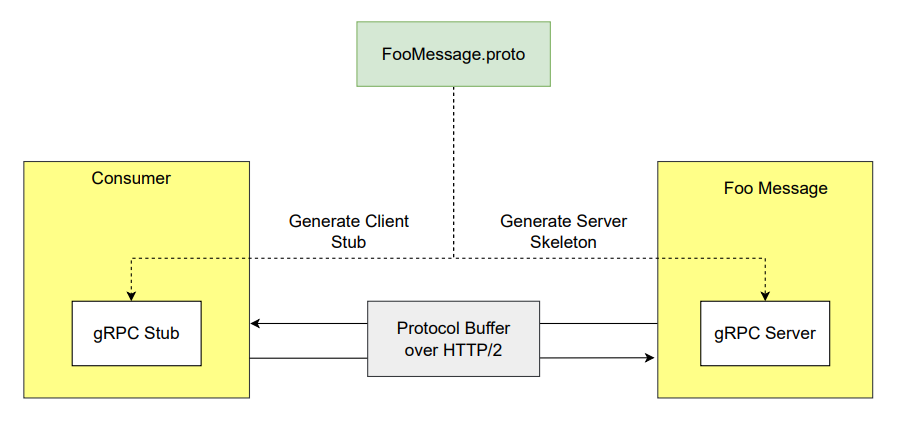
\includegraphics[width=0.8\textwidth]{images/grpc.png}
    \label{fig: grpcarchi}
\end{figure}

Quy trình giao tiếp giữa client và server trong gRPC diễn ra theo các bước chính:

\begin{enumerate}
    \item \textbf{Định nghĩa service}: Nhà phát triển định nghĩa service và message trong file \texttt{.proto}.
    \item \textbf{Sinh mã nguồn}: Công cụ protoc compiler tự động sinh ra các đoạn mã client stub và server skeleton từ file \texttt{.proto}.
    \item \textbf{Triển khai server}: Server triển khai các hàm xử lý thực tế dựa trên skeleton.
    \item \textbf{Gọi từ client}: Client sử dụng stub để gửi yêu cầu RPC tới server, truyền dữ liệu dưới dạng Protocol Buffers qua HTTP/2.
    \item \textbf{Nhận và xử lý response}: Server xử lý yêu cầu và gửi lại kết quả cho client theo đường truyền đã mở.
\end{enumerate}

gRPC hỗ trợ nhiều kiểu giao tiếp, bao gồm:

\begin{itemize}
    \item Unary RPC: Client gửi một request và nhận một response.
    \item Server streaming RPC: Client gửi một request và nhận nhiều response từ server.
    \item Client streaming RPC: Client gửi nhiều request và nhận một response từ server.
    \item Bidirectional streaming RPC: Client và server đồng thời gửi nhiều request và response.
\end{itemize}

\subsection{Ưu điểm và nhược điểm của gRPC}

Với kiến trúc dựa trên giao thức HTTP/2 và định dạng dữ liệu Protocol Buffers, gRPC mang lại nhiều ưu điểm nổi bật so với các mô hình API truyền thống. Trước hết, về mặt hiệu năng, gRPC cho phép truyền tải dữ liệu với độ trễ thấp và băng thông sử dụng tối ưu nhờ vào khả năng multiplexing, nén header và tuần tự hóa dữ liệu dạng nhị phân. Điều này đặc biệt quan trọng trong các hệ thống yêu cầu hiệu suất cao như truyền thông real-time, xử lý dữ liệu lớn hoặc giao tiếp giữa các dịch vụ back-end có tần suất cao.

Một ưu điểm đáng kể khác là tính đa nền tảng và đa ngôn ngữ. gRPC hỗ trợ nhiều ngôn ngữ lập trình phổ biến như Go, Java, Python, Node.js, C\#, giúp các hệ thống Microservices có thể được triển khai linh hoạt và dễ dàng tương tác giữa các thành phần viết bằng công nghệ khác nhau. Hơn nữa, việc sử dụng file định nghĩa dịch vụ \texttt{.proto} cho phép tự động sinh mã nguồn client và server, giúp giảm thiểu lỗi lập trình và tăng tốc độ phát triển.

Không chỉ dừng lại ở giao tiếp đơn giản dạng yêu cầu–phản hồi (request–response), gRPC còn hỗ trợ nhiều mô hình truyền thông nâng cao như server streaming, client streaming và bidirectional streaming. Những mô hình này rất phù hợp với các ứng dụng yêu cầu truyền dữ liệu liên tục hoặc theo thời gian thực.

Tuy nhiên, gRPC cũng tồn tại một số hạn chế nhất định. Do sử dụng HTTP/2 và định dạng dữ liệu nhị phân, việc debug thủ công trở nên khó khăn hơn so với các giao thức sử dụng JSON như REST. Ngoài ra, mặc dù gRPC hoạt động rất hiệu quả trong môi trường backend-to-backend, nhưng việc tích hợp trực tiếp với frontend (trình duyệt) còn hạn chế, do không phải mọi browser đều hỗ trợ đầy đủ HTTP/2 hoặc Protocol Buffers. Trong những trường hợp này, cần sử dụng gRPC-Web như một lớp trung gian, dẫn đến tăng độ phức tạp triển khai.

Cuối cùng, việc triển khai hạ tầng gRPC đòi hỏi các hệ thống và thiết bị hỗ trợ tốt HTTP/2 và TLS, điều này có thể là rào cản đối với các môi trường legacy hoặc mạng hạn chế về cấu hình.

\subsection{Ứng dụng thực tế của gRPC}

gRPC hiện được sử dụng rộng rãi trong nhiều hệ thống phân tán lớn yêu cầu độ trễ thấp, khả năng mở rộng và tính tương tác ngôn ngữ cao. Một số ứng dụng tiêu biểu bao gồm:

\begin{itemize}
    \item Giao tiếp giữa các Microservices trong hệ thống (backend-to-backend).
    \item Xây dựng backend cho mobile applications cần tối ưu băng thông.
    \item Hệ thống truyền tải dữ liệu real-time (video streaming, IoT telemetry).
\end{itemize}

Có thể nói, gRPC là một nền tảng RPC hiện đại, mang lại hiệu suất cao và khả năng tương tác đa nền tảng cho các hệ thống phần mềm phân tán. Với kiến trúc dựa trên HTTP/2 và Protocol Buffers, gRPC cung cấp một phương thức giao tiếp mạnh mẽ và tối ưu hơn nhiều so với các giải pháp truyền thống dựa trên HTTP/1.1. Việc ứng dụng gRPC phù hợp giúp các hệ thống Microservices nâng cao hiệu suất, tính mở rộng và khả năng quản lý hiệu quả trong các sản phẩm quy mô lớn.


\section{Chuẩn OpenTelemetry}

Trong các hệ thống phần mềm phân tán hiện đại, đặc biệt là kiến trúc Microservices, việc xây dựng khả năng quan sát (observability) toàn diện là một yêu cầu thiết yếu để đảm bảo vận hành ổn định và hiệu quả. Tuy nhiên, việc triển khai observability đồng nhất trên nhiều nền tảng và ngôn ngữ lập trình khác nhau đặt ra nhiều thách thức về tiêu chuẩn và tính tương thích.

\textbf{OpenTelemetry} \cite{otel} ra đời như một giải pháp tiêu chuẩn hóa, mã nguồn mở, được phát triển và duy trì bởi tổ chức Cloud Native Computing Foundation (CNCF). OpenTelemetry kết hợp những ưu điểm từ hai dự án tiền nhiệm là OpenTracing và OpenCensus, nhằm cung cấp một tập hợp đầy đủ các công cụ, API và SDK hỗ trợ thu thập, xử lý và xuất dữ liệu quan sát từ các hệ thống phân tán.

OpenTelemetry hỗ trợ ba loại dữ liệu giám sát chính như sau:

\begin{itemize}
    \item \textbf{Traces}: Ghi nhận hành trình xử lý của yêu cầu qua các dịch vụ.
    \item \textbf{Metrics}: Thu thập các chỉ số định lượng phản ánh hiệu suất hệ thống.
    \item \textbf{Logs}: Ghi lại sự kiện và trạng thái hoạt động chi tiết của từng thành phần.
\end{itemize}

Nhờ khả năng tiêu chuẩn hóa và đa nền tảng, OpenTelemetry trở thành lựa chọn phổ biến để tích hợp observability vào hệ thống Microservices, từ cấp độ ứng dụng tới hạ tầng.

\subsection{Thành phần của OpenTelemetry}

Hệ sinh thái OpenTelemetry được tổ chức thành các thành phần con, mỗi thành phần đảm nhiệm một vai trò cụ thể trong pipeline thu thập và xử lý dữ liệu giám sát:

\begin{itemize}
    \item \textbf{API}: Cung cấp tập hợp các giao diện lập trình ứng dụng (interface) cho phép các ứng dụng sinh ra và ghi nhận dữ liệu observability một cách thống nhất, độc lập với công nghệ backend cụ thể.
    
    \item \textbf{SDK}: Thư viện thực thi API OpenTelemetry, bao gồm các logic nội bộ để xử lý dữ liệu, thực hiện sampling (lấy mẫu), batching (gom nhóm) và chuẩn bị dữ liệu trước khi export.
    
    \item \textbf{Exporter}: Thành phần chịu trách nhiệm gửi dữ liệu đã thu thập tới các hệ thống lưu trữ và phân tích như \textbf{Jaeger}, \textbf{Prometheus}, \textbf{Zipkin}, \textbf{Elasticsearch} hoặc các nền tảng cloud observability như AWS X-Ray, Azure Monitor.
    
    \item \textbf{Collector}: Một dịch vụ trung gian có khả năng nhận dữ liệu từ nhiều nguồn, xử lý (processing, transformation) và phân phối tới các đích đến khác nhau. Collector hoạt động độc lập với ứng dụng, giúp giảm tải cho ứng dụng và cho phép thay đổi backend mà không cần sửa đổi mã nguồn.
\end{itemize}

\begin{figure}[H]{Kiến trúc tổng quan của OpenTelemetry}
    \centering
    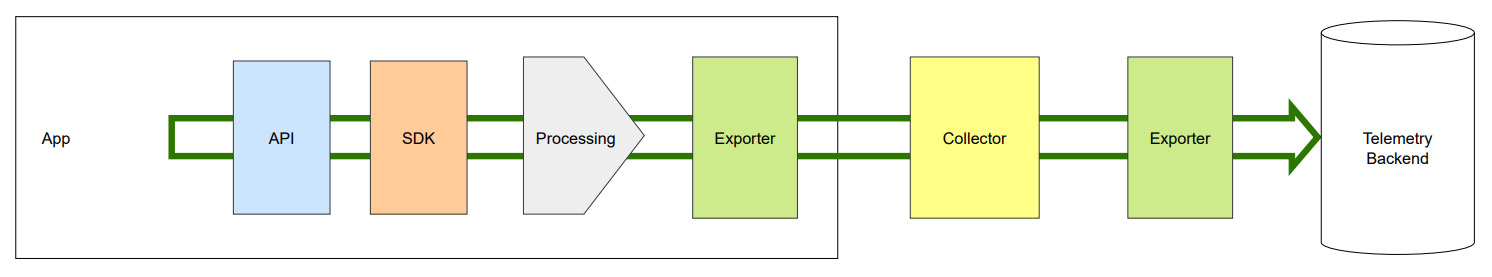
\includegraphics[width=0.85\textwidth]{images/otel.png}
    \label{fig:otel-archi}
\end{figure}

Hình~\ref{fig:otel-archi} mô tả chi tiết cách hoạt động của OpenTelemetry khi tích hợp vào một sản phẩm phần mềm. Quy trình thu thập và xử lý dữ liệu bằng OpenTelemetry diễn ra qua bốn giai đoạn chính:

\begin{enumerate}
    \item \textbf{Sinh dữ liệu}: Ứng dụng thực hiện các hoạt động nghiệp vụ và đồng thời sinh ra các logs, metrics và traces thông qua các API của OpenTelemetry.
    
    \item \textbf{Thu thập dữ liệu}: SDK OpenTelemetry trong ứng dụng sẽ tiếp nhận dữ liệu, áp dụng các chính sách sampling và tổ chức dữ liệu theo định dạng chuẩn.
    
    \item \textbf{Xử lý trung gian (tùy chọn)}: Nếu hệ thống triển khai OpenTelemetry Collector, dữ liệu sẽ được gửi tới Collector để thực hiện xử lý bổ sung như filtering, enriching, transforming.
    
    \item \textbf{Xuất dữ liệu}: Dữ liệu đã xử lý được gửi đến các backend observability như Prometheus (metrics), Jaeger (traces) hoặc hệ thống lưu trữ log để hiển thị, phân tích và cảnh báo.
\end{enumerate}

\subsection{Lợi ích của việc triển khai OpenTelemetry}

Việc tích hợp OpenTelemetry vào hệ thống mang lại nhiều lợi ích quan trọng:

\begin{itemize}
    \item \textbf{Tiêu chuẩn hóa observability}: Định nghĩa giao diện thu thập dữ liệu thống nhất trên toàn bộ hệ thống, giảm thiểu sự phụ thuộc vào công nghệ backend cụ thể.
    
    \item \textbf{Đa nền tảng và đa ngôn ngữ}: Hỗ trợ nhiều ngôn ngữ lập trình phổ biến như Go, Java, Python, Node.js, C\#, giúp dễ dàng áp dụng cho hệ sinh thái Microservices đa dạng.
    
    \item \textbf{Tăng khả năng tương tác công cụ}: Cho phép tích hợp liền mạch với nhiều hệ thống giám sát và phân tích mà không cần thay đổi mã nguồn.
    
    \item \textbf{Tối ưu hóa phát hiện và khắc phục sự cố}: Với khả năng tracing chi tiết và phân tích metrics thời gian thực, việc tìm kiếm nguyên nhân gốc rễ của lỗi (root cause analysis) trở nên nhanh chóng và hiệu quả hơn.
    
    \item \textbf{Giảm tải cho ứng dụng}: Việc tách việc thu thập, xử lý dữ liệu sang các Collector độc lập giúp ứng dụng giảm tải xử lý và tối ưu hiệu suất runtime.
\end{itemize}

\subsection{Ứng dụng của OpenTelemetry trong thực tế}

OpenTelemetry đã và đang được ứng dụng rộng rãi trong nhiều lĩnh vực khác nhau để nâng cao khả năng quan sát hệ thống:

\begin{itemize}
    \item \textbf{Giám sát hiệu suất hệ thống}: Thu thập metrics về độ trễ, throughput, lỗi để theo dõi và tối ưu hóa hiệu suất dịch vụ.
    
    \item \textbf{Phân tích nguyên nhân sự cố}: Dùng tracing để tái hiện luồng request qua nhiều service, xác định nhanh vị trí bottleneck hoặc điểm lỗi.
    
    \item \textbf{Tối ưu hóa trải nghiệm người dùng}: Phân tích hành vi user journey để điều chỉnh luồng xử lý, giảm độ trễ và tăng độ ổn định tương tác người dùng.
    
    \item \textbf{Tích hợp hệ thống cảnh báo tự động}: Kết nối dữ liệu metrics và traces với hệ thống cảnh báo để phát hiện bất thường và kích hoạt phản ứng nhanh chóng (incident response).
\end{itemize}

OpenTelemetry không chỉ là một bộ công cụ thu thập dữ liệu quan sát, mà còn là một tiêu chuẩn nền tảng để xây dựng các hệ thống phân tán hiện đại với khả năng quan sát mạnh mẽ, linh hoạt và mở rộng. Việc triển khai OpenTelemetry đóng vai trò then chốt trong hành trình phát triển các hệ thống Microservices bền vững, đáng tin cậy và dễ vận hành trong môi trường sản xuất thực tế.

\section{Distributed Tracing}
Distributed Tracing (DT), còn được gọi là phân tích yêu cầu phân tán, là một phương pháp được sử dụng để phân tích và giám sát các ứng dụng. Các ứng dụng phân tán, chẳng hạn như những ứng dụng dựa trên kiến trúc Microservices, làm cho việc phân tích nguyên nhân gốc rễ của các lỗi ứng dụng trở nên phức tạp hơn so với một ứng dụng nguyên khối (monolithic). Ví dụ, một dịch vụ front-end có thể gửi truy vấn đến một dịch vụ back-end để lấy dữ liệu mà người dùng yêu cầu. Dịch vụ back-end khi xử lý yêu cầu này, có thể gửi truy vấn đến rất nhiều các dịch vụ khác, và những dịch vụ này lại có thể gọi thêm các dịch vụ khác, để tổng hợp thông tin mà người dùng yêu cầu. Luồng yêu cầu này tiếp tục cho đến khi tất cả dữ liệu được thu thập và xử lý. Trong ví dụ trên, giả sử dịch vụ back-end đầu tiên gặp sự cố và không thể cung cấp dữ liệu được yêu cầu cho front-end. Sự cố này được nhóm phụ trách dịch vụ back-end đầu tiên phát hiện. Tuy nhiên, sự cố không phải do dịch vụ của họ gây ra, mà là do dịch vụ này không nhận được dữ liệu từ dịch vụ downstream của nó. Nhưng nhóm không có quyền truy cập vào dịch vụ downstream này. Kết quả là, nhóm không thể xác minh liệu dịch vụ đó có phải là nguyên nhân gốc rễ hay sự cố bắt nguồn từ một dịch vụ xa hơn trong chuỗi. Distributed Tracing giải quyết vấn đề này bằng cách ghi lại request đến services và cung cấp cái nhìn tổng quan về tất cả các yêu cầu từ dịch vụ này sang dịch vụ khác trong việc xử lý một yêu cầu từ người dùng.

\subsection{Các khái niệm cơ bản trong Distributed Tracing}
Distributed Tracing thường xoay quanh các khái niệm sau:
\begin{itemize}
    \item Trace: Đại diện cho toàn bộ hành trình của một yêu cầu xuyên qua hệ thống. Một trace bao gồm nhiều span.
    \item Span: Là một đơn vị công việc cụ thể trong hệ thống, ví dụ như một lời gọi API, truy vấn cơ sở dữ liệu, hoặc xử lý nghiệp vụ. Mỗi span ghi lại thông tin như thời gian bắt đầu, thời gian kết thúc, metadata liên quan,...
    \item Trace ID: Là định danh duy nhất cho một trace, dùng để liên kết các span liên quan với nhau.
    \item Span ID: Là định danh duy nhất của từng span.
    \item Parent Span / Child Span: Span có thể có quan hệ cha-con, biểu diễn quan hệ gọi giữa các dịch vụ.
\end{itemize}

Hình~\ref{fig:trace-span} dưới đây là sơ đồ đơn giản minh họa một trace gồm nhiều span:

 \begin{figure}[H]{Sơ đồ trace}
				\centering
				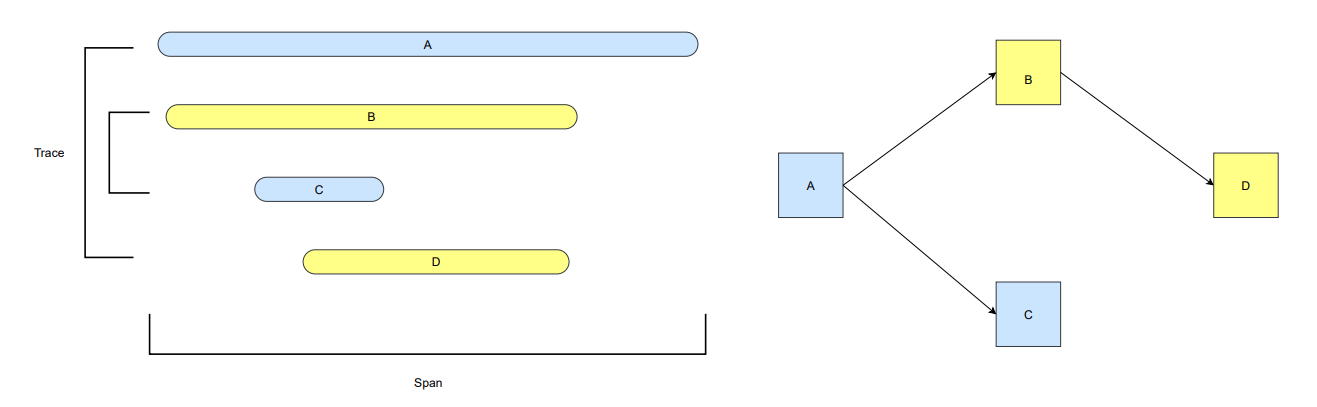
\includegraphics[width=14cm]{images/trace.png}
                \label{fig:trace-span}
	\end{figure} \\

    \textbf{Quy trình theo dõi phân tán sẽ bao gồm các bước như sau:}
    
\begin{itemize}
    \item Instrumentation (gắn mã theo dõi): Ứng dụng hoặc hệ thống cần được gắn mã để thu thập dữ liệu span (thường sử dụng các thư viện như OpenTelemetry).
    \item Propagation (truyền trace context): Các dịch vụ cần truyền ngữ cảnh trace (trace ID, span ID) qua header HTTP hoặc metadata để duy trì chuỗi liên kết giữa các span.
    \item Collection (thu thập): Dữ liệu trace được thu thập và gửi tới hệ thống lưu trữ/hiển thị như Jaeger, Zipkin, Datadog,...
    \item Visualization \& Analysis: Dữ liệu được trực quan hóa dưới dạng cây (tree) hoặc timeline để người vận hành dễ dàng phân tích.
\end{itemize}

\subsection{Tiêu chuẩn W3C Trace Context trong Distributed Tracing}

Distributed tracing là một kỹ thuật cốt lõi để theo dõi các yêu cầu (request) khi chúng đi qua nhiều dịch vụ khác nhau trong hệ thống Microservices. Để đảm bảo khả năng liên kết giữa các thành phần hệ thống được triển khai khác nhau hoặc sử dụng công nghệ khác nhau, việc chuẩn hóa thông tin trace trở nên cần thiết. 

Chuẩn W3C Trace Context \cite{tracectx} ra đời nhằm mục đích thống nhất cách thức truyền tải metadata liên quan đến tracing trong hệ thống phân tán. W3C Trace Context định nghĩa hai header HTTP chính: \texttt{traceparent} và \texttt{tracestate}. Bảng~\ref{tab:tracectx} bên dưới mô tả ý nghĩa của từng thành phần này. 

\begin{table}[H]{Các thành phần của chuẩn W3C Trace Context}
\centering
\begin{tabular}{|p{4cm}|p{10cm}|}
\hline
\textbf{Header} & \textbf{Ý nghĩa} \\
\hline
traceparent & Chứa thông tin Trace ID, Span ID và sampling flags cho trace hiện tại. \\
\hline
tracestate & Metadata bổ sung liên quan đến các vendor hoặc hệ thống cụ thể, hỗ trợ liên kết thông tin tracing mở rộng. \\
\hline
\end{tabular}
\label{tab:tracectx}
\end{table}

Header \texttt{traceparent} mang thông tin cơ bản về trace hiện tại, bao gồm Trace ID, Parent Span ID và sampling flags. Header này cho phép các thành phần hệ thống nhận biết một request thuộc về trace nào, và xác định mối quan hệ giữa các spans.

Header \texttt{tracestate} cho phép truyền tải thêm metadata mở rộng, phục vụ nhu cầu tùy chỉnh riêng của từng tổ chức hoặc nhà cung cấp công cụ.

Việc tuân thủ chuẩn W3C Trace Context giúp hệ thống có khả năng interoperability cao hơn, dễ dàng tích hợp với các công cụ phân tích observability phổ biến như OpenTelemetry, Jaeger, Zipkin và các hệ thống APM thương mại.

\subsection{Cơ chế Context Propagation trong OpenTelemetry}

Một trong những thành phần cốt lõi để thực hiện Distributed Trace chính là cơ chế truyền ngữ cảnh (Context Propagation), vốn được chuẩn hóa và hỗ trợ mạnh mẽ trong OpenTelemetry. Trong mô hình tracing của OpenTelemetry, mỗi đơn vị hoạt động trong hệ thống được đại diện bởi một \textit{Span}. Một chuỗi các span có liên hệ cha-con sẽ tạo thành một \textit{Trace}. Để kết nối các span lại với nhau, OpenTelemetry sử dụng một đối tượng gọi là \textbf{Context}, trong đó chứa thông tin định danh của các span đã được khởi tạo, chẳng hạn như trace ID và span ID. Hình~\ref{fig:ctxpropage} cung cấp cái nhìn tổng quan cách context được truyền giữa các services. Khi một dịch vụ (ví dụ: service A) gọi sang một dịch vụ khác (ví dụ: service B), Context hiện tại sẽ mang theo span ID của service A, và thông tin này sẽ được sử dụng để khởi tạo một span mới trong service B, với span A đóng vai trò là \textit{Parent Span}. Nhờ đó, toàn bộ chuỗi các lời gọi giữa các dịch vụ có thể được tái hiện dưới dạng một trace thống nhất.

\begin{figure}[H]{Sơ đồ context propagation}
				\centering
				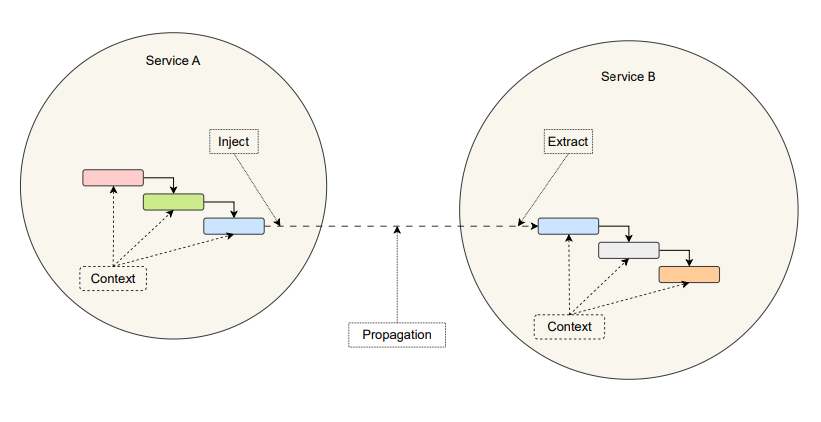
\includegraphics[width=14cm]{images/contextpropage.png}
                \label{fig:ctxpropage}
	\end{figure} \\

Cơ chế Propagation chính là phần chịu trách nhiệm truyền tải context giữa các thành phần trong hệ thống. Thông qua việc \textit{inject} và \textit{extract} Context vào trong các request (thường thông qua header HTTP hoặc metadata trong gRPC), OpenTelemetry giúp serialize và deserialize thông tin trace một cách tự động. Mỗi SDK hoặc middleware tích hợp OpenTelemetry sẽ đảm nhiệm vai trò này trong quá trình gửi và nhận dữ liệu. Với cơ chế này, khi một request được chuyển từ dịch vụ này sang dịch vụ khác, thông tin về trace context sẽ được bảo toàn, cho phép hệ thống phân tích dễ dàng toàn bộ luồng xử lý một cách chính xác.

Bên cạnh đó, OpenTelemetry tuân thủ tiêu chuẩn Trace Context của W3C, giúp đảm bảo tính tương thích giữa các công cụ observability khác nhau. Các thông tin như trace ID, span ID, sampling decision... đều được truyền theo định dạng thống nhất. Nhờ vậy, dù các dịch vụ trong hệ thống được viết bằng các ngôn ngữ lập trình khác nhau, hoặc sử dụng các thư viện khác nhau, quá trình propagation vẫn được duy trì hiệu quả.

Tóm lại, Context Propagation đóng vai trò thiết yếu trong việc xây dựng Distributed Tracing. Nhờ vào cơ chế này, OpenTelemetry có thể tái hiện chính xác toàn bộ hành trình của một yêu cầu trong hệ thống microservices, từ đó hỗ trợ các công cụ backend như Jaeger hay Zipkin phân tích, trực quan hóa và chẩn đoán lỗi một cách hiệu quả hơn.

    \chapter{PHÂN TÍCH THIẾT KẾ GIẢI PHÁP}
    \section{Phân tích yêu cầu}
    Giải pháp thu thập, xử lý và phân tích dữ liệu hành vi trong kiến trúc Microservices cần đáp ứng đầy đủ cả yêu cầu chức năng và phi chức năng để đảm bảo hiệu quả, độ tin cậy và khả năng áp dụng thực tế.

\subsection{Yêu cầu chức năng}
Giải pháp cần đảm bảo các chức năng chính sau:
\begin{itemize}
    \item \textbf{Thu thập dữ liệu:} Ghi nhận đầy đủ các yêu cầu HTTP từ phía người dùng gửi đến hệ thống, bao gồm thông tin về thời gian, phương thức, địa chỉ truy cập, endpoint và mã phản hồi,... .
    \item \textbf{Xử lý dữ liệu:} Tích hợp với OpenTelemetry để ghi nhận các truy vết (trace) của request khi đi qua nhiều services, từ đó xây dựng được bức tranh toàn cảnh về luồng xử lý trong hệ thống.
    \item \textbf{Phân tích và trực quan hóa dữ liệu:} Xử lý dữ liệu thu thập được để phân tích hành vi, xác định các xu hướng, điểm nghẽn, điểm lỗi của hệ thống và hiển thị kết quả thông qua giao diện trực quan phục vụ người quản trị hoặc nhà phát triển.
\end{itemize}

\subsection{Yêu cầu phi chức năng}
Bên cạnh các chức năng chính, hệ thống cũng cần đảm bảo các yêu cầu phi chức năng quan trọng như:
\begin{itemize}
    \item \textbf{Hiệu suất và khả năng mở rộng:} Giải pháp cần thu thập và xử lý khối lượng lớn dữ liệu hành vi được sinh ra từ nhiều dịch vụ. Đồng thời, kiến trúc phải hỗ trợ mở rộng dễ dàng theo nhu cầu thực tế.
    \item \textbf{Độ tin cậy và khả năng khôi phục:} Hệ thống cần hoạt động ổn định, có khả năng xử lý lỗi và phục hồi sau sự cố, đảm bảo tính liên tục của quá trình thu thập và phân tích dữ liệu.
\end{itemize}
 \newpage
	\section{Kiến trúc tổng thể}

Kiến trúc tổng thể của giải pháp được xây dựng xoay quanh một hệ thống Microservices. Hệ thống này gồm nhiều dịch vụ nhỏ giao tiếp với nhau, nhằm tái hiện các luồng nghiệp vụ trong hệ thống Microservices, đồng thời tạo ra dữ liệu hành vi người dùng và hành vi hệ thống để phục vụ cho việc thử nghiệm và đánh giá giải pháp.

Bên cạnh hệ thống trên, giải pháp bao gồm các thành phần chính được minh họa như Hình~\ref{fig:tongquangp} bên dưới. \textbf{Trigger module} được tích hợp vào các dịch vụ để ghi lại toàn bộ HTTP request của người dùng. \textbf{OTel Exporter module} được sử dụng để thu thập dữ liệu tracing nhằm theo dõi luồng xử lý của các request giữa các dịch vụ. Dữ liệu sau khi được thu thập sẽ được gửi bất đồng bộ qua \textbf{message broker}, giúp đảm bảo tính linh hoạt và không gây ảnh hưởng đến hiệu năng của hệ thống chính.

Dữ liệu từ message broker được xử lý và lưu trữ vào hai hệ thống cơ sở dữ liệu: \textbf{MongoDB}, sử dụng để lưu trữ dữ liệu hành vi theo dạng sự kiện, và \textbf{Elasticsearch}, phục vụ cho việc tìm kiếm dữ liệu logs nhanh chóng. Lớp phân tích phía sau bao gồm \textbf{Analystics API}, cung cấp các endpoint phục vụ truy vấn, phân tích và tổng hợp dữ liệu hành vi, và cuối cùng là \textbf{Frontend visualization}, một giao diện trực quan giúp hiển thị các góc nhìn quan trọng về cách người dùng tương tác hệ thống, và cách hệ thống xử lý, phản hồi yêu cầu người dùng.

Kiến trúc này đảm bảo tính thực tế, hỗ trợ kiểm tra tính khả thi cho giải pháp đề xuất, đồng thời có khả năng mở rộng và ứng dụng trong các hệ thống hiện hành.

            \begin{figure}[H]{Mô hình tổng quan giải pháp}
				\centering
				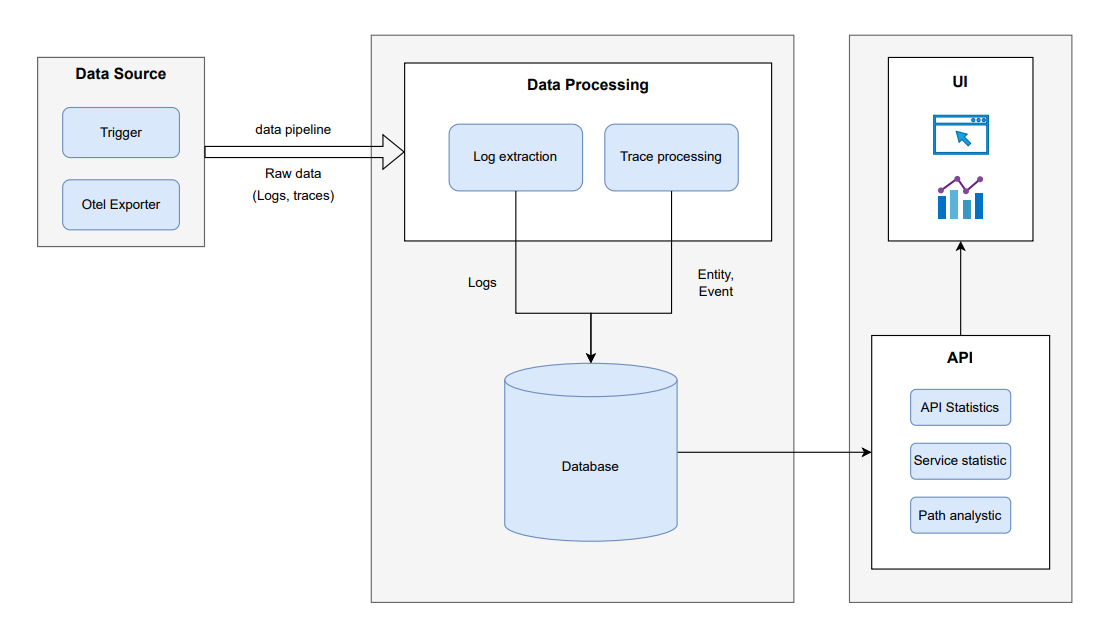
\includegraphics[width=14cm]{images/tongquan.png}
                \label{fig:tongquangp}
	\end{figure} \\

   \section{Phân tích và thiết kế chi tiết}

\subsection{Module thu thập dữ liệu}
\label{subsec:ttdl}

Để thu thập dữ liệu hành vi từ hệ thống Microservices, giải pháp sử dụng hai cơ chế chính: ghi lại thông tin HTTP request từ người dùng và tracing request giữa các dịch vụ. Trước tiên, các dịch vụ trong hệ thống được tích hợp một trigger module, ở đây là một HTTP middleware, có nhiệm vụ ghi lại toàn bộ thông tin HTTP request từ phía người dùng vào hệ thống, bao gồm các thông tin như endpoint, phương thức gọi (GET, POST,...), mã trạng thái phản hồi và thời gian xử lý,... . Middleware này được thiết kế lightweight và không gây ảnh hưởng đáng kể đến hiệu suất dịch vụ. Bên cạnh đó, việc xử lý một request từ người dùng cũng sinh ra log bên trong hệ thống. Với mỗi log loại này, ta sẽ thêm vào thông tin traceID và spanID để phục vụ việc truy vấn thống kê sau này.

Song song với đó, giải pháp cũng sử dụng OpenTelemetry như một chuẩn để thu thập dữ liệu tracing. Lý do chọn OpenTelemetry do đây là một open-source framework phổ biến, cung cấp đầy đủ các công cụ thu thâp dữ liệu telemetry, do đó việc tích hợp vào các hệ thống hiện hành hay triển khai cho các hệ thống mới được thực hiện dễ dàng, nhanh chóng và bảo mật. Tích hợp OpenTelemetry SDK vào từng dịch vụ giúp sinh ra các span, thể hiện từng bước xử lý trong chuỗi dịch vụ. Các span này được liên kết với nhau thông qua cơ chế context propagation — sử dụng các header như \texttt{trace-parent} và \texttt{baggage} trong mỗi HTTP request để truyền thông tin truy vết giữa các dịch vụ. Nhờ đó, có thể theo dõi đầy đủ đường đi của một request xuyên suốt toàn hệ thống. Dữ liệu thu thập được sẽ được chuẩn hóa dưới dạng JSON trước khi gửi đến module xử lý.

\subsection{Pipeline truyền dữ liệu}

Dữ liệu hành vi thu thập được từ middleware và OpenTelemetry sẽ được đưa đến module xử lý thông qua NATS – một message broker hiệu năng cao. Trong kiến trúc của giải pháp, NATS đóng vai trò trung tâm trong việc truyền tải dữ liệu bất đồng bộ, đảm bảo rằng việc ghi nhận dữ liệu không làm gián đoạn hoạt động của các dịch vụ chính. Giải pháp sử dụng NATS làm message broker thay vì Kafka hoặc RabbitMQ. Lý do lựa chọn được phân tích theo Bảng~\ref{tab:ssnats} như sau:

\begin{table}[H]{So sánh giữa NATS, Kafka và RabbitMQ}
\centering
\begin{tabular}{|p{3cm}|p{3cm}|p{3cm}|p{3cm}|}
\hline
\textbf{Tiêu chí} & \textbf{NATS} & \textbf{Kafka} & \textbf{RabbitMQ} \\
\hline
Độ trễ (Latency) & Rất thấp ($<1$ ms) & Trung bình (5–10 ms) & Thấp (1–5 ms) \\
\hline
Throughput & Cao (hàng triệu msg/s) & Rất cao (tối ưu cho batch) & Trung bình (10k–100k msg/s) \\
\hline
Độ phức tạp triển khai & Đơn giản & Cao (cluster, zookeeper) & Trung bình \\
\hline
Quản lý message & Lightweight (ephemeral) & Persistent storage mạnh mẽ & Persistent queue, phù hợp task queue \\
\hline
Phù hợp streaming nhỏ & Rất phù hợp & Phù hợp batch lớn & Phù hợp cho RPC/Task queue \\
\hline
\end{tabular}
\label{tab:ssnats}
\end{table}

Như vậy, với yêu cầu latency thấp, tốc độ xử lý cao cho các sự kiện hành vi nhỏ lẻ, đồng thời đơn giản trong triển khai để tránh các overhead không cần thiết, NATS là lựa chọn tối ưu cho giải pháp này.

Các thông điệp được gửi đến NATS sẽ được phân loại theo từng chủ đề (subjects), ví dụ: \texttt{logs.http} cho HTTP request logs, \texttt{logs.internal} cho logs bên trong hệ thống và \texttt{traces.service} cho dữ liệu tracing. Cấu trúc của mỗi message được chuẩn hóa và chứa đầy đủ metadata cần thiết như \texttt{timestamp}, \texttt{service\_name}, \texttt{trace\_id}, giúp dễ dàng xử lý ở module phía sau. Cơ chế publish-subscribe của NATS cho phép nhiều subscriber xử lý dữ liệu song song, nâng cao khả năng mở rộng của hệ thống. Trong trường hợp xảy ra lỗi hoặc mất kết nối, hệ thống hỗ trợ cơ chế retry tự động nhờ JetStream, đảm bảo độ tin cậy cao trong việc truyền dữ liệu.

\subsection{Module xử lý dữ liệu}
        \textbf{Dữ liệu loại 1: Logs}
        
        Với dữ liệu loại 1, sau khi nhận được HTTP request logs từ NATS server, logs sẽ được đi qua một filter để lọc các logs không có ý nghĩa cho việc phân tích như log của health check API, metadata API,... Sau đó logs tiếp tục đi qua một Mapper giúp lọc bỏ các field không cần thiết, giữ lại các field có ý nghĩa phân tích. Cuối cùng logs sau khi được chuẩn hóa sẽ được lưu vào MongoDB database dưới dạng event để phục vụ truy vấn time range. Internal log sẽ được lưu trữ vào Elasticsearch để phục vụ các truy vấn theo TraceID và SpanID. Bảng~\ref{tab:logmiddle} và Bảng~\ref{tab:loginternal} mô tả chi tiết data model được lưu dưới dạng event của 2 loại dữ liệu logs kể trên.

    \begin{table}[H]{Cấu trúc dữ liệu \texttt{log\_middleware\_event}}
\centering
\begin{tabular}{|p{4cm}|p{3.5cm}|p{7cm}|}
\hline
\textbf{Tên trường} & \textbf{Kiểu dữ liệu} & \textbf{Mô tả} \\
\hline
timestamp & Number & Thời điểm ghi nhận sự kiện (theo chuẩn thời gian quốc tế). \\
\hline
service\_name & String & Tên của service phát sinh log. \\
\hline
endpoint & String & API endpoint được gọi. \\
\hline
duration & Number & Thời gian xử lý request, tính bằng milliseconds. \\
\hline
query\_params & String & Tham số truy vấn đi kèm request, dạng JSON hoặc chuỗi URL-encoded. \\
\hline
request\_size & Number & Kích thước request gửi lên (đơn vị byte). \\
\hline
response\_size & Number & Kích thước response trả về (đơn vị byte). \\
\hline
user\_id & String & Mã định danh người dùng (nếu có). \\
\hline
user\_agent & String & Thông tin trình duyệt/thiết bị của người dùng. \\
\hline
trace\_id & String & Mã định danh trace dùng trong distributed tracing. \\
\hline
span\_id & String & Mã định danh span tương ứng với request hiện tại. \\
\hline
status\_code & Number & Mã trạng thái HTTP response. \\
\hline
error\_message & String & Thông điệp lỗi (nếu có). Nếu request thành công thì để null hoặc rỗng. \\
\hline
\end{tabular}
\label{tab:logmiddle}
\end{table}

   \begin{table}[H]{Cấu trúc dữ liệu \texttt{internal\_log}}
\centering
\begin{tabular}{|p{4cm}|p{3.5cm}|p{7cm}|}
\hline
\textbf{Tên trường} & \textbf{Kiểu dữ liệu} & \textbf{Mô tả} \\
\hline
timestamp & Number & Thời điểm ghi nhận log nội bộ. \\
\hline
traceID & String & Mã định danh trace chứa log này. \\
\hline
spanID & String & Mã định danh span nơi log này được ghi nhận. \\
\hline
message & String & Nội dung log (thường là thông điệp lỗi, cảnh báo hoặc thông tin nghiệp vụ). \\
\hline
\end{tabular}
\label{tab:loginternal}
\end{table}

        \textbf{Dữ liệu loại 2: Traces}
        
        Với dữ liệu loại 2, việc xử lý dữ liệu traces được xây dựng trên cơ sở các khái niệm mới về tracing và request flow. Trước hết ta sẽ đưa ra một vài nhận xét. Trong hệ thống Microservices, mỗi service cung cấp nhiều operation (gồm các hàm nội bộ và các API), và việc gọi các operation này sẽ tạo 1 span. Dữ liệu span bao gồm id, service và operation được gọi, timestamp và duration, parent span id,... Mỗi trace là tập hợp nhiều span cùng traceID dưới dạng cây, cấu trúc cây này thể hiện thứ tự gọi các service với nhau. Các trace có cùng dạng cây được xem như cùng một path hay một request flow. Một luồng nghiệp vụ có thể bao gồm nhiều path, và được xác định bởi việc đi qua 1 hoặc 2 service/operation cụ thể. Ví dụ nghiệp vụ thanh toán sẽ bao gồm các path đi qua operation /checkout của Checkout service. Điều này sẽ phụ thuộc vào cách định nghĩa các service của nhà phát triển phần mềm. Khi đó ta đi tới 2 khái niệm mới được đề cập bởi nhóm tác giả ở eBay \cite{gmta} như sau: \textbf{Hop} là abstraction của span, thể hiện việc gọi operation của service. \textbf{Path} là abstraction của trace, là tập hợp nhiều hop dưới dạng cây, thể hiện đường đi của request. Hình~\ref{fig:anhxa} mô tả chi tiết mối quan hệ giữa các đối tượng này.
        \begin{figure}[H]{Mô hình ánh xạ Hop, Path}
				\centering
				\includegraphics[width=14cm]{images/hinh5.png}
				\label{fig:anhxa}
	\end{figure} 

        Ở đây ta xét ví dụ sau: Giả sử ta có một hệ thống thương mại điện tử bao gồm các service sau:
        \begin{itemize}
            \item Service A - API Gateway: Xử lý yêu cầu từ người dùng.
            \item Service B - Order Service: Quản lý các đơn đặt hàng.
            \item Service C - Inventory Service: Kiểm tra tồn kho sản phẩm.
            \item Service D - Payment Service: Xử lý thanh toán.
        \end{itemize}

\textbf{Tình huống:} Một người dùng đặt hàng qua ứng dụng, hệ thống sẽ gọi các dịch vụ để xử lý đơn hàng.
\begin{itemize}
    \item Bước 1: Người dùng gửi yêu cầu đặt hàng. Người dùng gửi yêu cầu đến hệ thống qua Service A (API Gateway).
    \item Bước 2: Tạo đơn hàng. Service A gọi Service B (Order Service) để tạo một đơn hàng mới.
    \item Bước 3: Kiểm tra tồn kho. Sau khi đơn hàng được tạo, Service B gửi yêu cầu đến Service C (Inventory Service) để kiểm tra xem sản phẩm có trong kho hay không.
    \item Bước 4: Xử lý thanh toán. Nếu sản phẩm còn trong kho, Service B tiếp tục gửi yêu cầu đến Service D (Payment Service) để xử lý thanh toán cho đơn hàng.
    \item Bước 5: Trả kết quả cho người dùng. Cuối cùng, sau khi xử lý thành công tất cả các bước, Service A trả kết quả về cho người dùng, thông báo rằng đơn hàng đã được tạo thành công.
\end{itemize}

Trong ví dụ trên, trace data sẽ được ghi lại để theo dõi yêu cầu của người dùng đi qua các dịch vụ, mô tả ở Bảng~\ref{tab:traceexample} bên dưới.

\begin{table}[H]{Trace data example in Microservices}
\centering
\begin{tabular}{|c|c|c|c|c|c|}
\hline
\textbf{Span ID} & \textbf{Service} & \textbf{Operation} & \textbf{Parent Span ID} & \textbf{Duration (ms)} \\ 
\hline
 1 & API Gateway & Create Order & - & 120 \\ 
\hline
 2 & Order Service & Check Inventory & 1 & 50 \\ 
\hline
 3 & Inventory Service & Get Stock & 2 & 30 \\ 
\hline
 4 & Order Service & Payment & 1 & 60 \\ 
\hline
 5 & Payment Service & Process Payment & 4 & 40 \\ 
\hline
\end{tabular}
\label{tab:traceexample}
\end{table}

 Nhìn vào Hình~\ref{fig:tracetree} bên dưới, hình vuông là các service và các elip cùng màu là các operation của service đó. Mỗi hình elip đại diện cho 1 span sinh ra từ việc gọi operation, và trace là biểu diễn dạng cây của các span. Khi này, việc operation gọi operation sẽ được xem là 1 hop, ví dụ \textit{Create Order} gọi \textit{Check Inventory}, và path đại diện cho cấu trúc cây của traces, thể hiện thứ tự gọi các operation, 2 trace có cùng cấu trúc cây được xem như cùng một path.
  \begin{figure}[H]{Biểu diễn dạng cây của trace}
				\centering
				\includegraphics[width=9cm]{images/hinh7.png}
				\label{fig:tracetree}
	\end{figure} 

   Ở đây, ta coi service, operation, hop và path là các entity chính trong hệ thống. Các entity này sẽ cố định không thay đổi trừ khi có thêm requirement hoặc requirement cũ thay đổi. Mỗi span sinh ra từ OpenTelemetry sẽ chứa 2 loại thông tin: thông tin của entity như ID, name; và thông tin event của entity đó như timestamp, duration, error. Ta sẽ thu thập các event liên quan tới các entity này để lưu vào MongoDB phục vụ cho các truy vấn time range. Việc xử lý và lưu trữ riêng 2 loại thông tin trên giúp việc truy vấn aggregate hiệu quả hơn, đồng thời giảm trùng lặp dữ liệu, tiết kiệm không gian lưu trữ dữ liệu. Data model được lưu dưới dạng event được mô tả ở Bảng~\ref{tab:pathevent} và Bảng~\ref{tab:hopevent} như sau:
   
    \begin{table}[H]{Cấu trúc dữ liệu \texttt{path\_event}}
\centering
\begin{tabular}{|p{4cm}|p{3.5cm}|p{7cm}|}
\hline
\textbf{Tên trường} & \textbf{Kiểu dữ liệu} & \textbf{Mô tả} \\
\hline
path\_id & String & Mã định danh duy nhất cho luồng xử lý (path) tương ứng với một trace. \\
\hline
timestamp & Number & Thời điểm ghi nhận sự kiện xảy ra với path. \\
\hline
has\_error & Boolean & Đánh dấu liệu path có chứa lỗi ở bất kỳ bước nào hay không. \\
\hline
\end{tabular}
\label{tab:pathevent}
\end{table}

   \begin{table}[H]{Cấu trúc dữ liệu \texttt{hop\_event}}
\centering
\begin{tabular}{|p{4cm}|p{3.5cm}|p{7cm}|}
\hline
\textbf{Tên trường} & \textbf{Kiểu dữ liệu} & \textbf{Mô tả} \\
\hline
timestamp & Number & Thời điểm hop được thực hiện trong trace. \\
\hline
hop\_id & String & Mã định danh cho một hop – tương ứng với lời gọi giữa hai operation trong hệ thống. \\
\hline
duration & Number & Thời gian thực thi của hop, tính bằng milliseconds. \\
\hline
has\_error & Boolean & Cho biết hop này có phát sinh lỗi hay không. \\
\hline
\end{tabular}
\label{tab:hopevent}
\end{table}
        
        Hình~\ref{fig:traceprocess} mô tả cách thức hoạt động của luồng xử lý trace data. Module xử lý sẽ subscribe NATS server để nhận span data. Span sẽ được buffer trong một khoảng thời gian trong các bucket được xác định bởi TraceID trước khi được đưa vào xử lý. Mục đích là để thu thập được toàn bộ span mà một request sinh ra, với điều kiện ở đây là các trace phải kết thúc sau một thời gian nhất định. Từ mỗi trace, ta dựng một Directed Acyclic Graph (DAG) với các node là các span, 2 span có cạnh liên kết nếu chúng có quan hệ cha-con. Để so sánh xem 2 DAG có cùng path hay không, ta sử dụng thuật toán để tạo ra PathID với mỗi cây thu được, 2 cây cùng PathID được xem là cùng một path. Thuật toán chi tiết được mô tả trong đoạn mã \ref{alg:pathid} bên dưới. Sau khi tính pathID, ta kiểm tra xem trong database đã có pathID này chưa, nếu không thì sẽ thêm mới path vào database, cùng với đó là các event liên quan đến path như timestamp, error, duration phục vụ cho việc phân tích.
        
         \begin{figure}[H]{Trace processing}
				\centering
				\includegraphics[width=14cm]{images/hinh6.png}
				\label{fig:traceprocess}
	\end{figure} 
    \newpage
    \begin{lstlisting}[language=psedo, caption={Thuật toán tạo PathId}, label={alg:pathid}]
        SpanHash(root, level):
            hash = HashCode(root.serviceName) + HashCode(root.operationName) 
                    + level x 31
            for child in root.children:
                hash+=SpanHash(child, level + 1)
    
            return hash
    \end{lstlisting}

\subsection{Lưu trữ dữ liệu}

Hệ thống sử dụng kết hợp hai công nghệ lưu trữ là MongoDB và Elasticsearch để phục vụ hai mục đích khác nhau. MongoDB được sử dụng để lưu trữ dữ liệu hành vi dưới dạng tài liệu JSON, rất phù hợp với cấu trúc dữ liệu linh hoạt từ các HTTP logs và traces. Mỗi tài liệu trong MongoDB đại diện cho một request hoặc một trace, bao gồm các thông tin như thời gian, dịch vụ xử lý, người dùng, tham số,... cho phép dễ dàng truy xuất theo time-range để phục vụ phân tích thống kê.

Trong khi đó, Elasticsearch được dùng để lưu trữ logs với khả năng truy vấn nhanh và phân tích theo thời gian thực. Dữ liệu trong Elasticsearch được tổ chức dưới dạng index với các trường đã được phân tích (analyzed fields), hỗ trợ mạnh mẽ các truy vấn phức tạp, thống kê và visualization. Elasticsearch được cấu hình với chiến lược indexing và sharding hợp lý để đảm bảo hiệu năng truy xuất và khả năng mở rộng khi dữ liệu tăng nhanh. Ngoài ra, Elasticsearch cũng cần tích hợp các cơ chế backup định kỳ và chính sách retention để kiểm soát dung lượng lưu trữ và đảm bảo an toàn dữ liệu, ví dụ chỉ lưu trữ dữ liệu trong 6 tháng gần nhất.

\subsection{API phân tích}

Để cung cấp khả năng truy xuất và khai thác dữ liệu, hệ thống triển khai một lớp \textit{Analytics API} với các REST API endpoints. Các API này cho phép thực hiện nhiều loại truy vấn khác nhau như: thống kê số lượng request theo thời gian, phân tích thời gian phản hồi trung bình của các dịch vụ, truy vết một yêu cầu cụ thể từ người dùng, hoặc tái hiện luồng gọi dịch vụ dưới dạng cây (trace tree). Mục tiêu của việc phân tích là đưa ra các góc nhìn quan trọng cho đội ngũ phát triển về cách mà người dùng sử dụng tính năng của sản 
phẩm, cũng như luồng nghiệp vụ bên trong của hệ thống. Các truy vấn được chia thành các loại chính:
\begin{itemize}
    \item Service Query: bao gồm các truy vấn thống kê các service được sử dụng nhiều nhất hoặc ít nhất, hoặc thông tin chi tiết về một service cụ thể về các khía cạnh như tần suất gọi, tần suất lỗi,... của các API mà service cung cấp.
    \item API Query: bao gồm các truy vấn thống kê các API được sử dụng nhiều nhất hoặc ít nhất, hoặc thông tin chi tiết về một API cụ thể như tần suất gọi, thời gian phản hồi,... .
    \item Path query: bao gồm các truy vấn liên quan tới Path, đại diện cho một luồng nghiệp vụ cụ thể. Một path sẽ được xác định bằng các service/operation nó đi qua. Sau khi tìm kiếm, nhà phát triển có thể xem thông tin chi tiết của 1 path như luồng xử lý, tần suất gọi trong một khoảng thời gian cụ thể.
    \item Trace query: bao gồm các truy vấn liên quan tới việc tìm kiếm trace như tìm kiếm theo pathID, hoặc truy vấn thông tin chi tiết một trace, các lỗi xảy ra bên trong trace, log tương ứng với trace đó.
\end{itemize}

\chapter{TRIỂN KHAI GIẢI PHÁP}

\section{Môi trường triển khai}

Giải pháp được triển khai đánh giá trong môi trường thử nghiệm, sử dụng cấu hình phần cứng và phần mềm phổ biến. Cụ thể, hệ thống chạy trên máy chủ với cấu hình CPU 4 cores, RAM 8GB và ổ cứng SSD 50GB.

Về công nghệ, hệ thống Microservices được phát triển bằng ngôn ngữ Go, sử dụng framework Echo cho HTTP server và gRPC cho giao tiếp nội bộ. MongoDB và Elasticsearch được dùng cho lưu trữ dữ liệu, trong khi NATS đóng vai trò là message broker. Giao diện frontend được phát triển bằng React và kết nối trực tiếp với REST API phân tích. Quá trình triển khai và quản lý dịch vụ được thực hiện thông qua Docker và Docker Compose, cho phép tái tạo môi trường dễ dàng và nhanh chóng.

\section{Hệ thống Microservices}

Hệ thống Microservices sử dụng trong khóa luận gồm nhiều dịch vụ nhỏ đại diện cho các thành phần phổ biến trong một ứng dụng thực tế, ở báo cáo này ta giả lập nghiệp vụ thanh toán cho hệ thống ecommerce. Hệ thống gồm 5 service nghiệp vụ: \texttt{Checkout service, Order service, Inventory service, Address service, Payment service}. Các dịch vụ này được container hóa và giao tiếp với nhau thông qua HTTP hoặc gRPC. Yêu cầu người dùng sẽ gọi trực tiếp tới \texttt{Checkout service}, với HTTP endpoint là \texttt{/user-checkout}. \texttt{Checkout service} sẽ gọi gRPC tới các dịch vụ liên quan để xử lý yêu cầu, thông tin luồng xử lý sẽ được ghi lại thông qua dữ liệu logs và trace. Kiến trúc tổng quan của hệ thống được mô tả như Hình~\ref{fig:ms-archi} bên dưới.

\begin{figure}[H]{Kiến trúc của hệ thống Microservices}
				\centering
				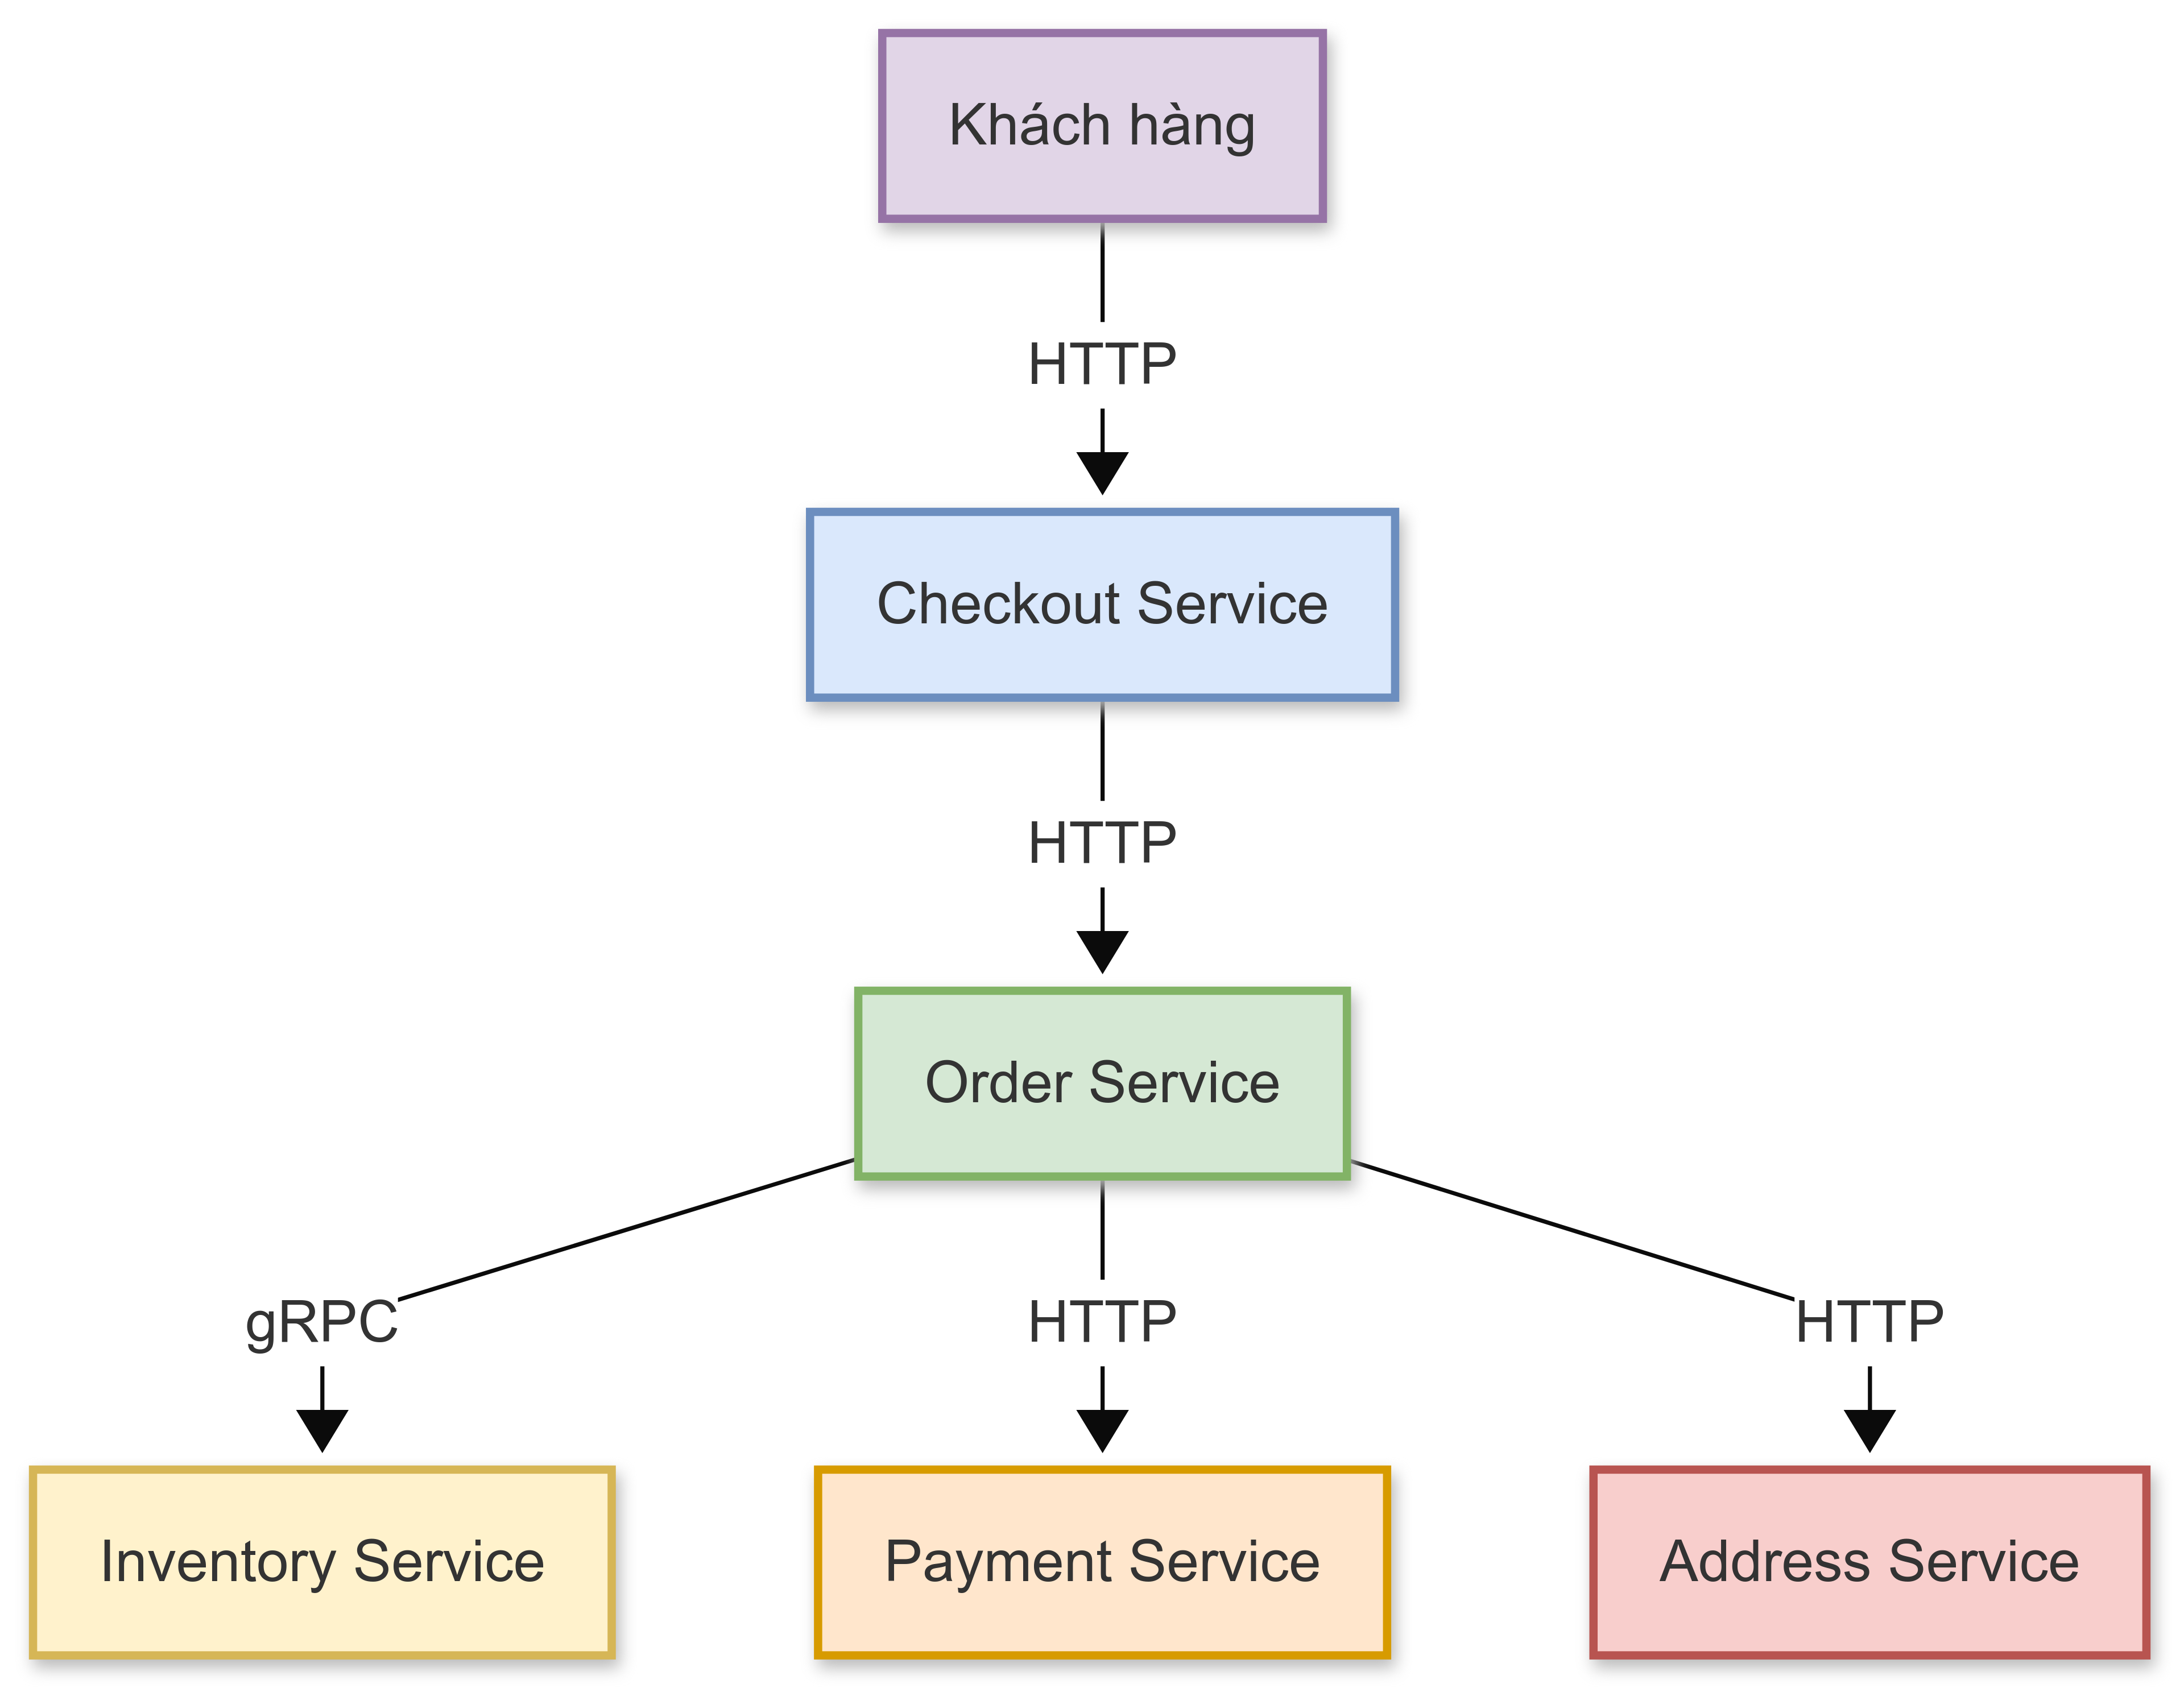
\includegraphics[width=14cm]{images/msa-tongquan.png}
				\label{fig:ms-archi}
	\end{figure} 

\section{Tích hợp module thu thập dữ liệu}
\subsection{Tích hợp middleware logging}
Middleware logging được cài đặt trực tiếp trong các dịch vụ để ghi lại toàn bộ HTTP request. Middleware này hoạt động như một lớp trung gian giữa server và route handler, ghi nhận các thông tin như thời gian gọi API, phương thức, đường dẫn, mã trạng thái, IP client, và thời gian phản hồi.

Các log được định dạng theo cấu trúc JSON với đầy đủ metadata và được gửi tới NATS dưới subject \texttt{logs.http}. Việc tích hợp middleware được thực hiện bằng cách khai báo nó trong cấu hình server của từng dịch vụ, đảm bảo mỗi request đều được ghi nhận mà không ảnh hưởng hiệu năng tổng thể.

Việc logging bên trong hệ thống cũng được cấu hình thêm thông tin trace context vào log để phục vụ debugging, bao gồm traceID và spanID. Các log này sẽ được truyền vào NATS pipeline qua subject \texttt{logs.internal}, thông qua logstash để lưu trữ vào elasticsearch.

\subsection{Tích hợp OpenTelemetry}

Hệ thống Microservices tích hợp OpenTelemetry để thu thập, xử lý và phân tích dữ liệu xuyên suốt tất cả các dịch vụ. Việc triển khai tuân theo một mẫu nhất quán trên tất cả các service nghiệp vụ để đảm bảo khả năng quan sát đồng nhất.

Mỗi service khởi tạo một OpenTelemetry tracer trong quá trình khởi động thông qua thư viện tracing chung mà giải pháp cung cấp. Việc khởi tạo sẽ cấu hình tracer với tên service hiện tại và kết nối đến telemetry backend thông qua NATS.

Đối với giao tiếp dựa trên HTTP giữa các dịch vụ, hệ thống sử dụng instrumented HTTP client đã được đóng gói như một thư viện mà giải pháp cung cấp. Hàm này đóng gói HTTP transport tiêu chuẩn với công cụ OpenTelemetry để đảm bảo ngữ cảnh theo dõi được truyền trong các header HTTP. Đối với giao tiếp dựa trên gRPC, hệ thống sử dụng các interceptor mà OpenTelemetry cung cấp từ thư viện chuẩn cho cả phía client và server.

Web framework Echo được sử dụng bởi tất cả các dịch vụ được tích hợp với middleware OpenTelemetry \texttt{otelecho.Middleware("service-name")}, tự động tạo spans cho các yêu cầu HTTP đến.

Mỗi operation được tạo có thể thêm thông tin vào spans bằng các thuộc tính liên quan như thuộc tính của input, output. Ví dụ, trong phương thức CreateOrder của Order service, spans được tạo với các thuộc tính như ID người dùng và số lượng mặt hàng. Xử lý lỗi được tích hợp vào spans bằng cách ghi lại lỗi và thiết lập các thuộc tính lỗi thích hợp. Các sự kiện quan trọng trong operation được ghi lại bằng Otel API \texttt{span.AddEvent()}.

Hệ thống kết hợp logs với traces bằng cách bao gồm TraceID và SpanID trong các bản ghi log, đảm bảo rằng logs có thể được liên kết với các traces tương ứng để gỡ lỗi và phân tích toàn diện. Điều này đạt được bằng cách trích xuất span context và thêm thông tin vào các bản ghi log như đã trình bày ở phần~\ref{subsec:ttdl}.

Việc tích hợp OpenTelemetry toàn diện này cho phép quan sát chi tiết hành vi, hiệu suất và điều kiện lỗi của hệ thống thương mại điện tử, tạo điều kiện thuận lợi cho việc gỡ lỗi hiệu quả, tối ưu hóa hiệu suất và hiểu biết về hệ thống.

\section{Triển khai NATS message broker}

NATS server được cài đặt và cấu hình trên môi trường Docker, đảm bảo khả năng kết nối giữa các dịch vụ trong mạng nội bộ. Các Microservices sử dụng NATS client (tương ứng với ngôn ngữ lập trình) để publish dữ liệu log và trace lên các subject cụ thể. Trong hệ thống thương mại điện tử trên, NATS message broker đóng vai trò quan trọng như một thành phần trung tâm cho việc truyền tải dữ liệu Telemetry và dữ liệu log. Việc triển khai NATS được thực hiện thông qua một container riêng biệt trong môi trường Docker. Mỗi service đều được cấu hình để thiết lập kết nối đến NATS trong quá trình khởi động thông qua hàm \texttt{logging.InitNATS()} mà giải pháp cung cấp, cho phép gửi dữ liệu log và telemetry. Đặc biệt, NATS được tích hợp với thư viện ghi log của các service thông qua một custom writer \texttt{NATSLogWriter} của giải pháp, giúp tập trung hóa việc thu thập log từ tất cả các dịch vụ vào một điểm duy nhất. Bên cạnh đó, NATS cũng đóng vai trò quan trọng trong việc vận chuyển dữ liệu OpenTelemetry từ các dịch vụ đến module xử lý. Kiến trúc này giúp cải thiện khả năng quan sát toàn diện của hệ thống, tránh ảnh hưởng tới hiệu suất xử lý nghiệp vụ ban đầu thông qua xử lý bất đồng bộ. Các subject chính bao gồm \texttt{logs.http}, \texttt{traces.service}, và \texttt{log.internal}. NATS cũng hỗ trợ khả năng lưu trữ message tự động thông qua JetStream extension trong trường hợp mất kết nối với thành phần xử lý của giải pháp.

\section{Đánh giá giải pháp}

\subsection{Throughput của Pipeline}
Throughput được định nghĩa là số lượng message được xử lý thành công qua pipeline trong một đơn vị thời gian, thường tính bằng message/giây. Để đo metric này, hệ thống được cấu hình để ghi nhận số lượng message được gửi (publish) và xử lý (consume) tại các service sử dụng thư viện Prometheus.

Thử nghiệm được tiến hành với dữ liệu log và trace được gửi đồng thời từ nhiều Microservices. Kết quả đo trên môi trường thực nghiệm cho thấy hệ thống có khả năng xử lý trung bình \textbf{1,200 message/giây}, với độ dao động nhỏ khi tăng số lượng request đồng thời. Biểu đồ Hình~\ref{fig:thput} theo dõi từ Grafana dựa trên truy vấn Prometheus \texttt{rate(pipeline\_messages\_consumed\_total[1m])} thể hiện tốc độ ổn định của pipeline trong khoảng thời gian 10 phút, kể cả khi có các burst traffic ngắn hạn.

\begin{figure}[H]{Biểu đồ throughput pipeline theo thời gian}
				\centering
				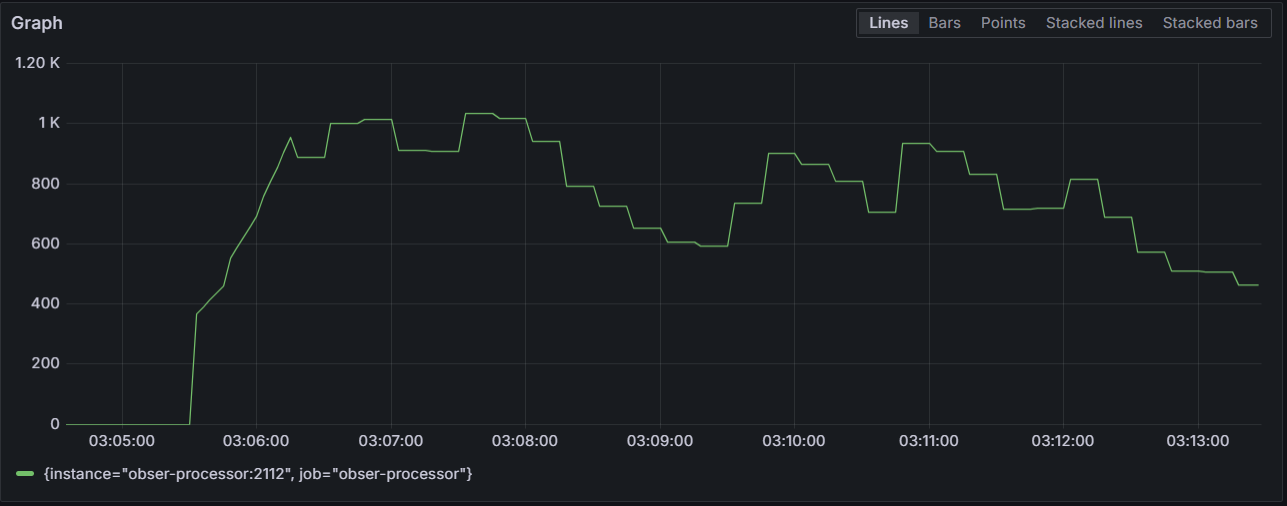
\includegraphics[width=10cm]{images/throughtput-pipeline.png}
                \label{fig:thput}
	\end{figure} 

\subsection{Overhead hệ thống}
Overhead được đo bằng độ trễ trung bình khi thêm middleware logging và OpenTelemetry instrumentation so với hệ thống không thu thập dữ liệu. Kết quả được tổng hợp ở Bảng~\ref{tab:overhead}cho thấy:

\begin{itemize}
    \item Middleware HTTP logging gây tăng trung bình \textbf{3-5ms} mỗi request.
    \item Instrumentation OpenTelemetry thêm khoảng \textbf{5-10ms}, tùy thuộc vào độ sâu của trace.
    \item Tổng overhead trung bình là \textbf{8-15ms/request}, nằm trong ngưỡng chấp nhận được đối với các hệ thống không yêu cầu thời gian thực nghiêm ngặt.
\end{itemize}

Việc sử dụng batching và non-blocking I/O trong pipeline giúp giảm thiểu ảnh hưởng của việc thu thập dữ liệu đến hiệu năng chung của hệ thống.

\begin{table}[H]{Tổng hợp overhead hệ thống khi thu thập dữ liệu hành vi}
    \centering
    \begin{tabular}{|c|c|}
        \hline
        \textbf{Thành phần} & \textbf{Độ trễ trung bình} \\
        \hline
        Middleware Logging & 3–5ms \\
        OpenTelemetry Instrumentation & 5–10ms \\
        \hline
        \textbf{Tổng cộng} & \textbf{8–15ms} \\
        \hline
    \end{tabular}
    \label{tab:overhead}
\end{table}

\chapter{THỰC NGHIỆM}

Phần thực nghiệm nhằm đánh giá khả năng áp dụng và hiệu quả của giải pháp thu thập, xử lý và phân tích dữ liệu hành vi trong môi trường hệ thống microservices thực tế. Các kịch bản thực nghiệm được xây dựng xoay quanh hai nhóm chính: phân tích hành vi người dùng và phân tích hành vi hệ thống. Thông qua các tình huống cụ thể, nhóm tác giả minh họa cách giải pháp hỗ trợ Product Manager và developer nhanh chóng truy xuất, phân tích và khai thác dữ liệu từ hệ thống, từ đó cải thiện hiệu suất vận hành, giảm thiểu thời gian xử lý lỗi và nâng cao trải nghiệm người dùng. Nội dung chương này sẽ trình bày chi tiết quy trình thực nghiệm, bao gồm các ví dụ minh họa, kết quả trực quan (hình ảnh, số liệu) và các phân tích rút ra được từ quá trình áp dụng giải pháp.

\section{Phân tích hành vi người dùng}
\textbf{Tình huống 1:} Một nền tảng thương mại điện tử cung cấp các API cho phép đối tác bên thứ ba tích hợp sản phẩm và dịch vụ của họ. Gần đây, nền tảng này nhận thấy sự chậm trễ trong việc xử lý đơn hàng và muốn xác định nguyên nhân. Sử dụng giải pháp trên, Product Manager truy xuất thông tin về số lần gọi đến từng API (Hình~\ref{fig:api-stat}), thời gian phản hồi và thông tin về đối tác sử dụng API, từ đó xác định các API có tần suất sử dụng cao (Hình~\ref{fig:most-used-api}) và thời gian phản hồi chậm (Hình~\ref{fig:latencyapi}), gây tắc nghẽn trong quá trình xử lý đơn hàng. Người quản lý lúc này có thể liên hệ đội phát triển service hay API đó để tối ưu hoặc sửa lỗi mã nguồn, hoặc yêu cầu đội quản lý hạ tầng cung cấp thêm tài nguyên cho service được sử dụng nhiều bởi người dùng. Giải pháp giúp nhanh chóng tìm ra các điểm nghẽn trong sản phẩm, cải thiện hiệu suất tổng thể và giảm thời gian xử lý đơn hàng, nâng cao trải nghiệm người dùng và tăng sự hài lòng của đối tác.

\begin{figure}[H]{Thống kê sử dụng API}
				\centering
				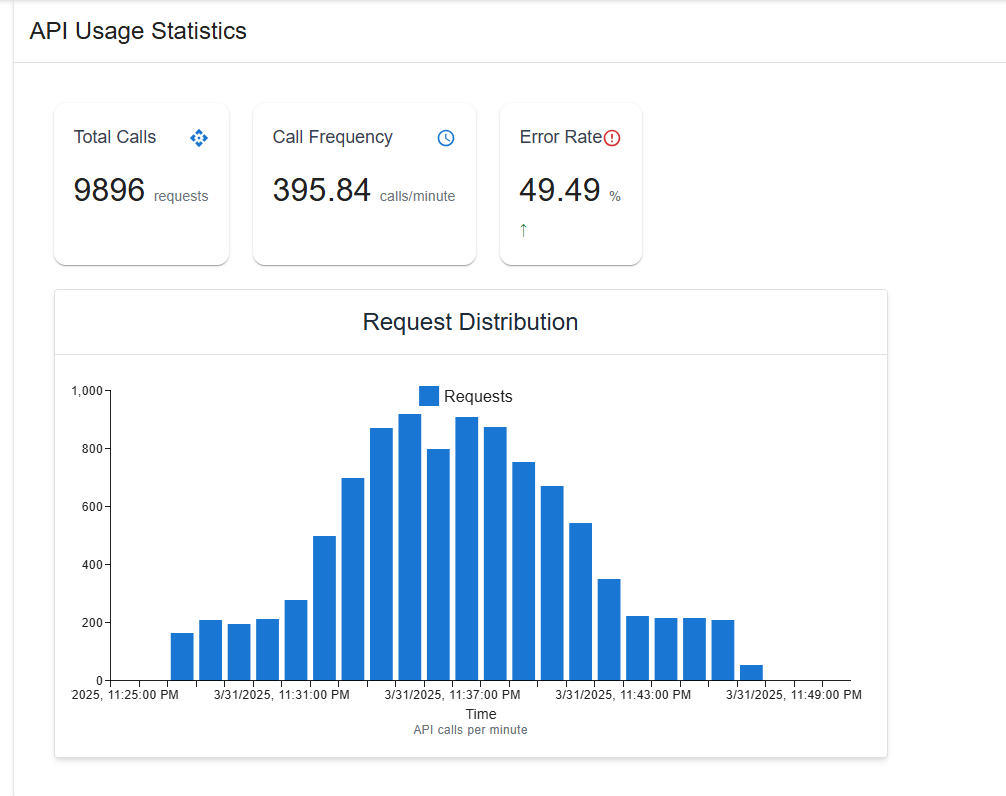
\includegraphics[width=14cm]{images/api-stat.png}
				\label{fig:api-stat}
	\end{figure} \\
\begin{figure}[H]{Danh sách các API có độ trễ cao}
				\centering
				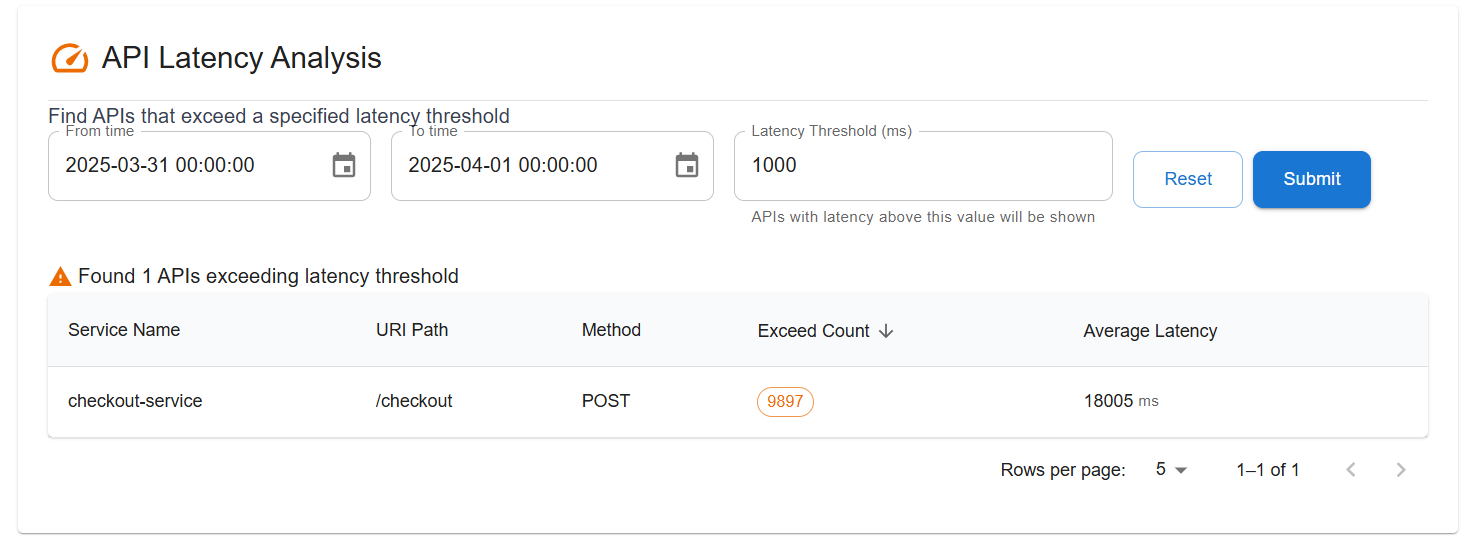
\includegraphics[width=14cm]{images/api-latency-threshold.png}
				\label{fig:latencyapi}
	\end{figure} \\
\begin{figure}[H]{Danh sách các API được gọi nhiều nhất}
				\centering
				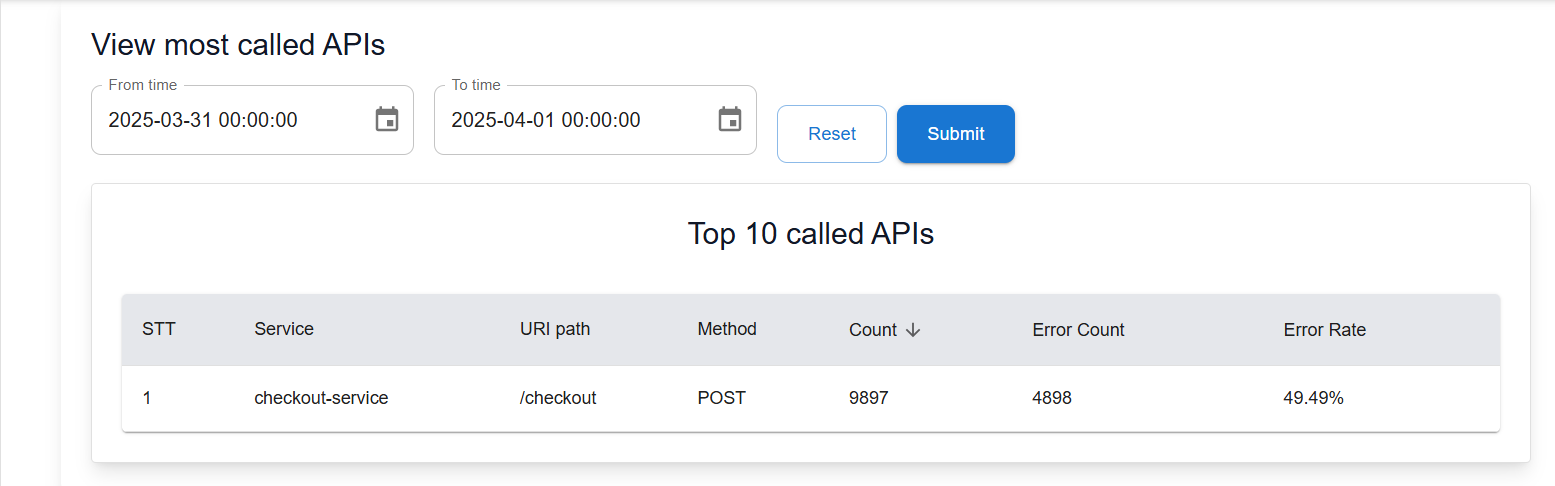
\includegraphics[width=14cm]{images/api-most-use.png}
				\label{fig:most-used-api}
	\end{figure} \\

\section{Phân tích hành vi hệ thống}
\subsection{Hiểu về kiến trúc hệ thống}
\textbf{Tình huống 2:} Hệ thống Microservices trong doanh nghiệp luôn là một hệ thống lớn với luồng nghiệp vụ phức tạp, việc hiểu và có cái nhìn tổng quát về hệ thống luôn là thách thức lớn đối với nhà phát triển, đặc biệt là người mới tham gia vào dự án. Với giải pháp này, việc tiếp cận và làm quen với hệ thống sẽ trở nên nhanh chóng, tiết kiệm thời gian và công sức. Một developer A mới gia nhập vào dự án ecommerce muốn tìm hiểu về luồng nghiệp vụ thanh toán của hệ thống. Sử dụng giải pháp, A tìm kiếm tất cả các path tương ứng với nghiệp vụ trên, ví dụ tất cả các path đi qua payment service. Giải pháp lúc này sẽ cung cấp cái nhìn tổng quan nhất của luồng nghiệp vụ như luồng xử lý, các service phụ thuộc vào payment service, như Hình~\ref{fig:paymentflow} bên dưới. Điều này giúp tiết kiệm rất nhiều thời gian và công sức đào tạo nhân viên mới, giúp họ tập trung vào phát triển luồng nghiệp vụ một cách hiệu quả.

\begin{figure}[H]{Sơ đồ luồng nghiệp vụ payment}
				\centering
				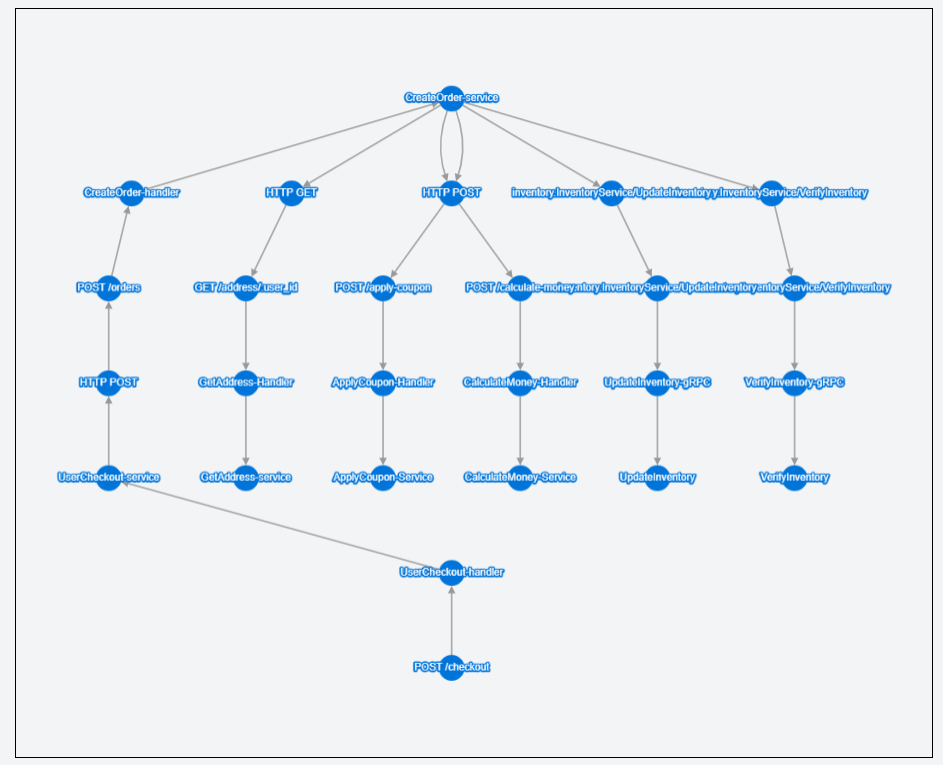
\includegraphics[width=14cm]{images/tim-kiem-path.png}
				\label{fig:paymentflow}
	\end{figure} \\

\subsection{Phục vụ debugging}
\textbf{Tình huống 3:} Việc bảo trì và sửa lỗi trong hệ thống Microservices luôn là thách thức rất lớn đối với các nhà phát triển và tiêu tốn chi phí rất lớn đối với doanh nghiệp. Để có thể tìm ra nguyên nhân gốc rễ vấn đề, developer sẽ phải quan sát thông tin tất cả các service liên quan tới nghiệp vụ đó. Sử dụng giải pháp này sẽ giúp developer nhanh chóng tìm ra nguyên nhân gốc rễ vấn đề, từ đó sửa lỗi nhanh và hiệu quả hơn. Ví dụ developer B được thông báo luồng nghiệp vụ tạo đơn hàng hiện tại đang có tỉ lệ lỗi cao bất thường. Sử dụng giải pháp, B chỉ cần tìm kiếm tất cả các path đi qua operation \texttt{/create-order} của Order service. Khi xem chi tiết thông tin 1 path trong khoảng thời gian hiện tại, B nhận thấy luồng gọi downstream xuống service \texttt{inventory} với operation \texttt{/verify-inventory} bị lỗi (Hình~\ref{fig:trace-present}), do đó B nhanh chóng xác định được phạm vi lỗi. Để tìm kiếm nguyên nhân gây ra lỗi, B có thể xem tất cả các trace của path đó, khi xem chi tiết 1 trace và đọc log sinh ra từ operation \texttt{/verify-inventory} (Hình~\ref{fig:trace-log}), B nhận thấy lỗi là từ việc viết sai câu lệnh truy vấn vào inventory database. B nhanh chóng sửa lại lỗi để khắc phục vấn đề nêu trên.

\begin{figure}[H]{Biểu diễn trace dạng timeline và graph}
				\centering
                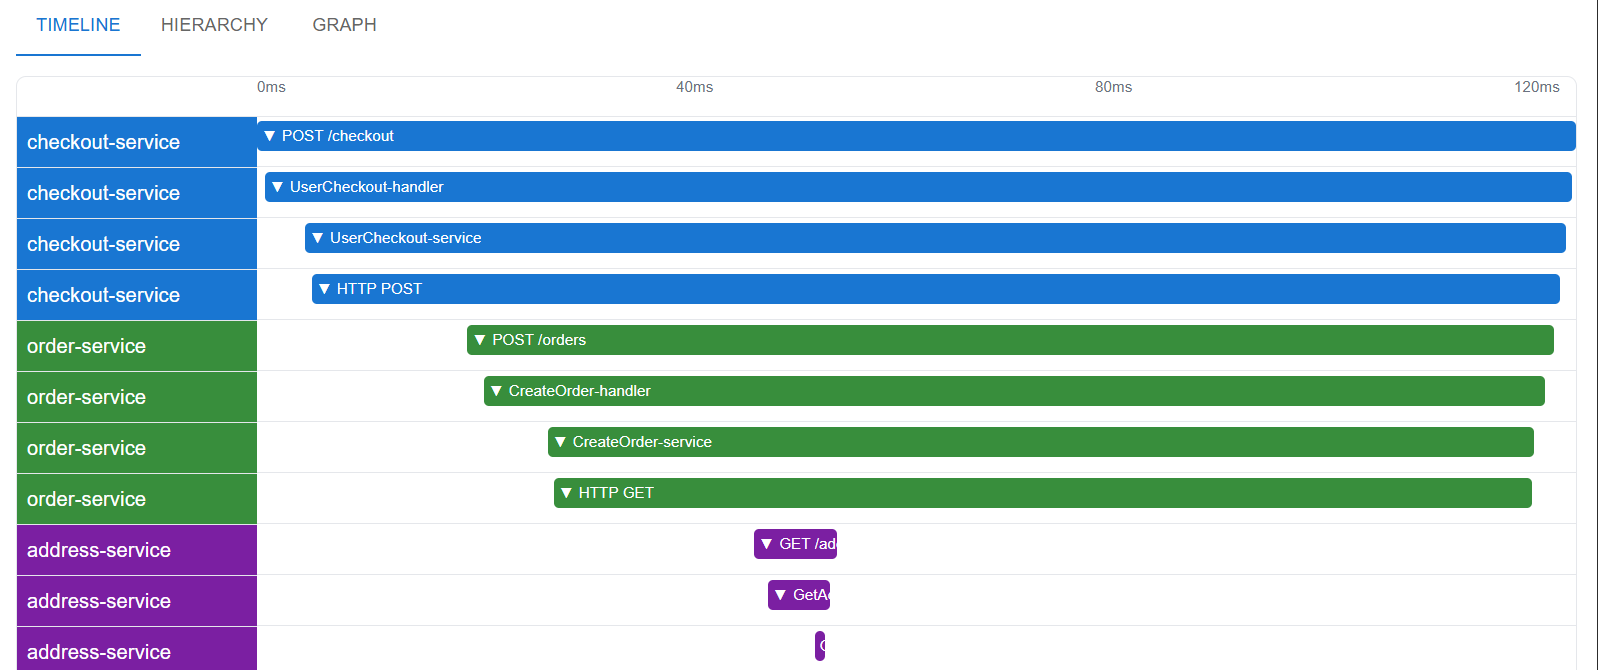
\includegraphics[width=14cm]{images/trace-timeline.png}
				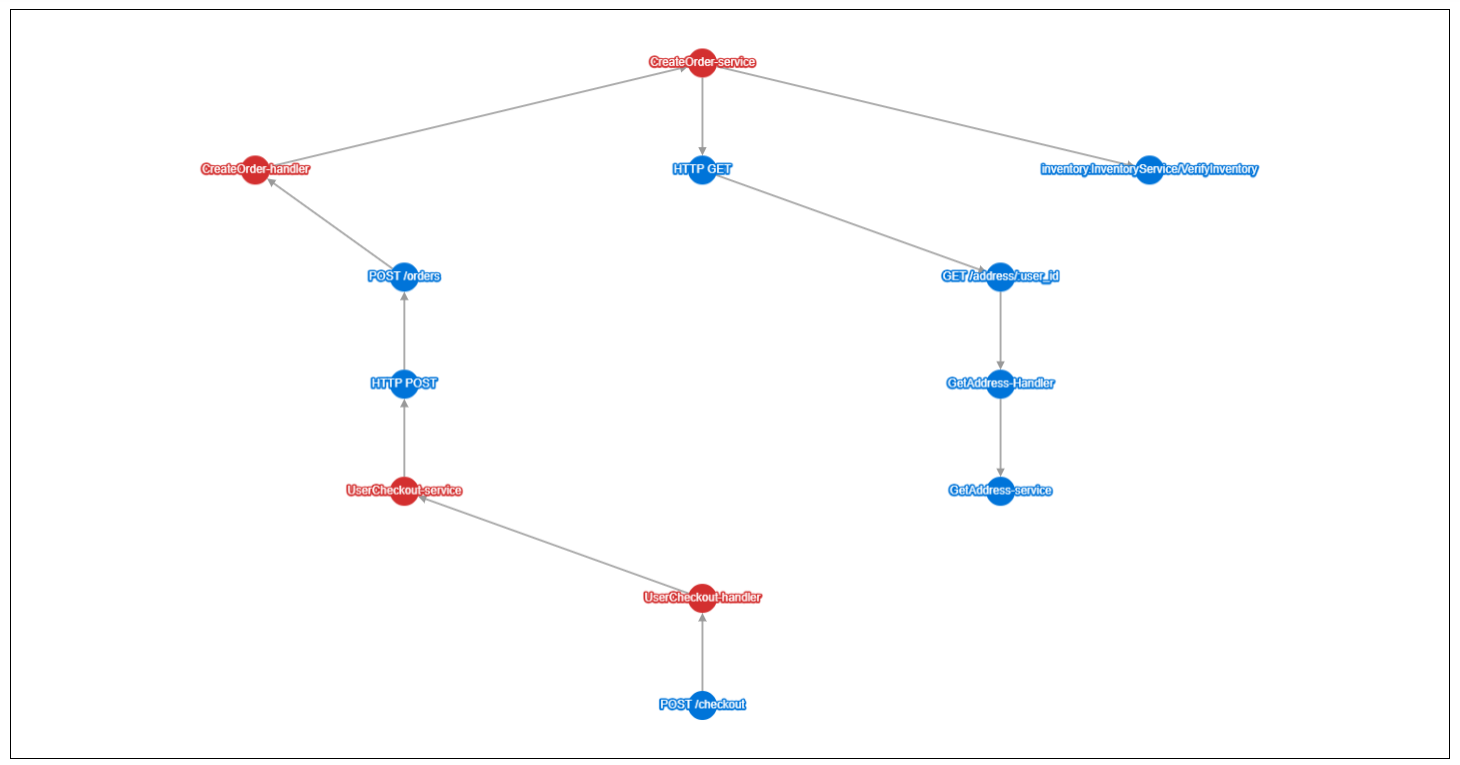
\includegraphics[width=14cm]{images/trace-flow.png}
                \label{fig:trace-present}
	\end{figure} \\

\begin{figure}[H]{Xem logs của order operation}
				\centering
				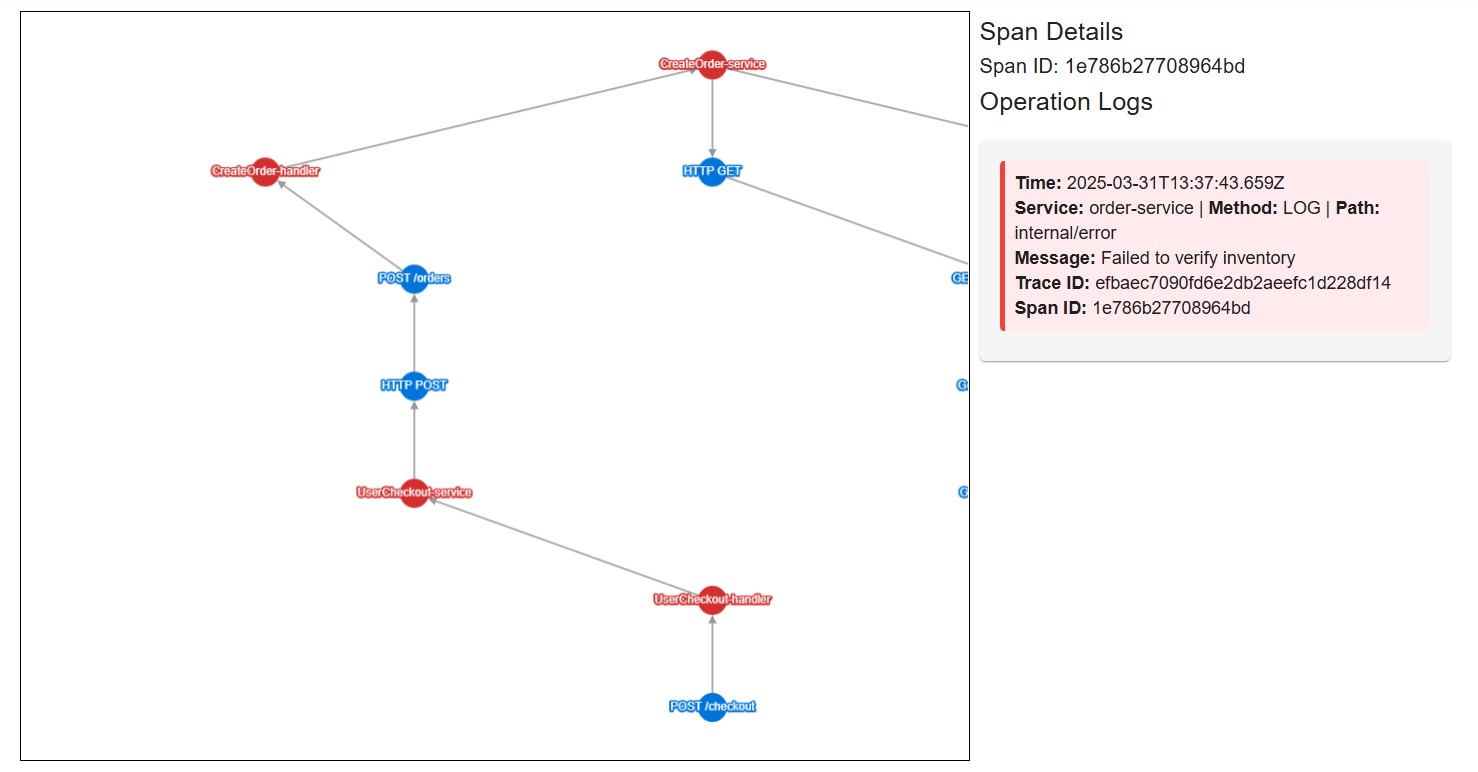
\includegraphics[width=14cm]{images/trace-logs.png}
                \label{fig:trace-log}
	\end{figure} \\

\chapter{KẾT LUẬN VÀ ĐỊNH HƯỚNG PHÁT TRIỂN}
\section{Kết luận}
Trong khuôn khổ nghiên cứu này, giải pháp thu thập và phân tích dữ liệu hành vi cho hệ thống Microservices đã được triển khai thành công. Hệ thống không chỉ cung cấp khả năng thu thập dữ liệu hành vi người dùng qua HTTP requests và hệ thống qua tracing, mà còn hỗ trợ phân tích và trực quan hóa dữ liệu này một cách hiệu quả. Các thành phần chính của hệ thống, bao gồm middleware logging, OpenTelemetry, NATS message broker, MongoDB, Elasticsearch và API phân tích, đã được tích hợp và triển khai thành công để cung cấp một giải pháp hoàn chỉnh cho việc thu thập, xử lý và phân tích dữ liệu hành vi trong các hệ thống Microservices. Giải pháp đã đạt được các mục tiêu cơ bản nhất dựa trên yêu cầu đặt ra ban đầu:

\begin{itemize}
\item Tích hợp module thu thập dữ liệu hành vi của người dùng và hệ thống trong môi trường Microservices, đảm bảo tính chính xác và hiệu suất cao.
\item Thiết kế pipeline xử lý dữ liệu để đảm bảo khả năng truyền tải nhanh chóng, mở rộng linh hoạt và giảm độ trễ trong quá trình xử lý.
\item Phát triển API và giao diện phân tích thống kê trực quan những góc nhìn quan trọng trong hệ thống cho các nhà phát triển ứng dụng, cung cấp công cụ hỗ trợ giảm chi phí bảo trì, sửa lỗi, tập trung phát triển các tính năng phần mềm mang lại giá trị cao cho người dùng.
\end{itemize}

Giải pháp này mang lại một mô hình tổng thể cho việc phân tích hành vi người dùng và hành vi hệ thống trong kiến trúc Microservices, qua đó cung cấp cái nhìn sâu sắc về hoạt động của hệ thống. Mô hình này tích hợp nhiều công nghệ hiện đại như OpenTelemetry để thu thập tracing, NATS cho messaging, MongoDB và Elasticsearch cho lưu trữ và tìm kiếm dữ liệu, tạo thành một hệ sinh thái hoàn chỉnh phục vụ cho việc phân tích hành vi.

Điều đặc biệt ở giải pháp này là khả năng triển khai một cách end-to-end, từ thu thập dữ liệu hành vi qua middleware và tracing, cho đến xử lý và phân tích dữ liệu, cuối cùng là việc trực quan hóa kết quả cho người dùng qua giao diện web. Giải pháp này mang lại sự linh hoạt và hiệu quả trong việc triển khai và phát triển các hệ thống Microservices hiện đại.

Mặc dù giải pháp đã đạt được nhiều kết quả khả quan, nhưng vẫn tồn tại một số hạn chế. Đầu tiên, hệ thống hiện tại chỉ được triển khai trong môi trường Microservices demo, với quy mô và phạm vi khá hạn chế. Điều này có thể ảnh hưởng đến khả năng mở rộng và áp dụng vào các hệ thống sản xuất với quy mô lớn hơn.

Bên cạnh đó, các công nghệ được chọn, như MongoDB và Elasticsearch, có thể gặp phải một số vấn đề về hiệu suất khi dữ liệu và truy vấn ngày càng trở nên phức tạp. Hệ thống chưa giải quyết được hoàn toàn các vấn đề về tối ưu hóa khi lượng dữ liệu lớn và yêu cầu phân tích phức tạp. Một số tính năng như phát hiện bất thường (anomaly detection) và dự đoán xu hướng hành vi vẫn chưa được tích hợp vào giải pháp.

\section{Định hướng phát triển}

Để nâng cao hiệu quả thu thập, xử lý và phân tích dữ liệu hành vi trong hệ thống Microservices, giải pháp đề xuất sẽ tiếp tục được mở rộng theo nhiều hướng phát triển trong tương lai. Những định hướng này không chỉ nhằm tối ưu hóa hiệu suất hệ thống, mà còn hướng tới việc mở rộng phạm vi dữ liệu quan sát, tăng cường khả năng mở rộng linh hoạt và đảm bảo tính ổn định trong môi trường vận hành thực tế.

Trước hết, hệ thống sẽ áp dụng các chiến lược tối ưu hóa xử lý luồng dữ liệu streaming nhằm cải thiện hiệu suất trong điều kiện dữ liệu phát sinh liên tục với tốc độ cao. Việc sử dụng cơ chế đệm tạm thời (buffering) cho phép hệ thống hấp thụ đột biến lưu lượng dữ liệu đầu vào, giảm tải cho các bước xử lý tiếp theo, đồng thời tạo điều kiện thuận lợi cho việc gom nhóm dữ liệu (batching). Kỹ thuật batching giúp giảm số lần truy cập cơ sở dữ liệu, tiết kiệm tài nguyên hệ thống và tăng throughput xử lý tổng thể. Bên cạnh đó, để đảm bảo tính ổn định khi hệ thống bị quá tải, cơ chế kiểm soát backpressure sẽ được tích hợp nhằm giới hạn tốc độ tiêu thụ, tạm dừng nhận sự kiện mới khi buffer đầy và đưa các sự kiện chưa xử lý kịp thời vào hàng chờ phụ để xử lý sau, tránh mất mát dữ liệu.

Về mặt độ tin cậy và khả năng mở rộng, hệ thống hướng đến việc triển khai cơ chế retry tự động với chiến lược exponential backoff nhằm xử lý các lỗi tạm thời trong quá trình lưu trữ hoặc truyền tải dữ liệu. Các sự kiện không thể xử lý sau nhiều lần retry sẽ được chuyển vào Dead Letter Queue (DLQ) để lưu trữ và xử lý sau. Đồng thời, kiến trúc hệ thống cũng được thiết kế theo hướng scale-out horizontal, cho phép tăng số lượng instance của các thành phần xử lý như Data Consumer hoặc API Server theo nhu cầu thực tế. Các chỉ số vận hành như CPU, số lượng message pending hay thời gian phản hồi sẽ là cơ sở để kích hoạt quá trình auto-scaling, đảm bảo hệ thống luôn đáp ứng tốt các đợt tải cao như thời điểm quảng bá sản phẩm hoặc mở rộng người dùng nhanh chóng.

Bên cạnh các cải tiến về kỹ thuật xử lý và vận hành, giải pháp cũng định hướng mở rộng phạm vi dữ liệu hành vi được thu thập và phân tích. Không chỉ dừng lại ở các truy vấn HTTP hay tracing hệ thống, dữ liệu log từ các dịch vụ backend, các chỉ số tài nguyên như CPU, bộ nhớ, hay hành vi người dùng từ ứng dụng mobile và thiết bị IoT cũng sẽ được tích hợp vào pipeline phân tích. Điều này giúp xây dựng một bức tranh toàn diện hơn về trạng thái hệ thống và hành vi sử dụng thực tế.

Một hướng phát triển tiềm năng khác là ứng dụng các phương pháp học máy (machine learning) vào quá trình phân tích dữ liệu hành vi. Việc sử dụng các mô hình học máy không chỉ cho phép phát hiện bất thường trong hoạt động của hệ thống và hành vi người dùng mà còn hỗ trợ phân tích xu hướng và dự đoán tương tác trong tương lai. Đây là nền tảng để tiến tới việc tự động hóa phân tích dữ liệu và cá nhân hóa trải nghiệm người dùng một cách hiệu quả.

Ngoài ra, việc tích hợp hệ thống với các công cụ DevOps và CI/CD hiện đại là một trong những mục tiêu quan trọng nhằm tối ưu hóa quy trình vận hành. Thông qua tự động hóa pipeline triển khai, kiểm thử và giám sát hiệu suất, hệ thống sẽ đảm bảo khả năng phản ứng linh hoạt với thay đổi, rút ngắn thời gian đưa tính năng mới ra thị trường và nâng cao độ ổn định vận hành. Cuối cùng, hệ thống sẽ được mở rộng khả năng tích hợp với các nền tảng giám sát và phân tích phổ biến như Prometheus, Grafana hay các observability platform hiện đại, nhằm xây dựng một hệ sinh thái giám sát – phân tích toàn diện, sẵn sàng triển khai trong môi trường sản xuất thực tế với độ tin cậy cao.



\begin{thebibliography}{9}
% \begin{bibsection}{Tiếng Việt}

% \end{bibsection}

\begin{bibsection}{}
\bibitem{openapi} OpenAPI Standard, \textit{https://www.openapis.org/}.
\bibitem{grpc} gRPC, \textit{https://grpc.io/}.
\bibitem{otel} OpenTelemetry Standard, \textit{https://opentelemetry.io/}.
\bibitem{tracectx} W3C Trace Context Standard, \textit{https://www.w3.org/TR/trace-context/} 
\bibitem{natsio} NATS.io, \textit{https://nats.io/}.
\bibitem{zipkin} Zipkin, \textit{https://zipkin.io/}.
\bibitem{jaeger} Jaeger, \textit{https://www.jaegertracing.io}.
\bibitem{martin} Martin Kleppmann, \textit{Designing Data-Intensive Applications: The Big Ideas Behind Reliable, Scalable, and Maintainable Systems}, 1st Edition.
\bibitem{Microservices} Sam Newman, \textit{Building Microservices: Designing Fine-Grained Systems}, 1st Edition.
\bibitem{gmta} Xiaofeng Guo, Xin Peng, Hanzhang Wang, Wanxue Li, Huai Jiang, Dan Ding, Tao Xie, and Liangfei Su. 2020. \textit{Graph-Based Trace Analysis for Microservices Architecture Understanding and Problem Diagnosis.} In Proceedings of the 28th ACM Joint European Software Engineering Conference and Symposium on the Foundations of Software Engineering (ESEC/FSE ’20), November 8–13, 2020, Virtual Event, USA.
\bibitem{dapper} Benjamin H. Sigelman, Luiz André Barroso, Mike Burrows, Pat Stephenson, Manoj Plakal, Donald Beaver, Saul Jaspan, and Chandan Shanbhag. 2010. \textit{Dapper, a Large-Scale Distributed Systems Tracing Infrastructure}. Technical Report. Google, Inc. https://research.google.com/archive/papers/dapper-2010-1.pdf.
\bibitem{uba} Roman Mysiuk, Oleksii Kononenko, Andriy Svystovych, Oleksii Ozhyhov. 2024. \textit{User Behavior Analysis Using Web-based Machine Learning Features: New Solutions for IT Business}. Path of Science.2024. Vol. 10. No 5.
\bibitem{sysbe} Michael Jackson. 2017. \textit{Engineering by Software: System Behaviours as Components}. The Open University. September 2017.
\bibitem{tracegroup} Adrita Samanta, Henry Han. 2023. \textit{Visualizing Distributed Traces in Aggregate}. MIT PRIMES, 2023.

\bibitem{canopy} J. Kaldor, J. Mace, M. Bejda, E. Gao, W. Kuropatwa, J. O’Neill, K. W. Ong, B. Schaller, P. Shan, B. Viscomi, V. Venkataraman, K. Veeraraghavan, and Y. J. Song. \textit{Canopy: An end-to-end performance tracing and analysis system}. In Proceedings of the
26th Symposium on Operating Systems Principles, SOSP ’17, New York, NY, USA, 2017. Association for Computing Machinery.

\bibitem{trainticket} Xiang Zhou, Xin Peng, Tao Xie, Jun Sun, Chenjie Xu, Chao Ji, Wenyun Zhao. 2018. \textit{Benchmarking Microservices Systems for Software Engineering Research}. In ICSE ’18 Companion: 40th International Conference on Software Engineering Companion, May 27-June 3, 2018, Gothenburg, Sweden. ACM, New York, NY, USA, 2 pages. \textit{https://doi.org/10.1145/3183440.3194991}.

\bibitem{faultanalysis} Xiang Zhou, Xin Peng, Tao Xie, Jun Sun, Chao Ji, Wenhai Li, and Dan Ding. \textit{Fault Analysis and Debugging of Microservices
Systems: Industrial Survey, Benchmark System, and Empirical Study}. IEEE Transaction on software engineering, vol.14, no.8, August 2018.

\bibitem{microtrend} P. D. Francesco, I. Malavolta, and P. Lago. \textit{Research on architecting Microservices: Trends, focus, and potential for industrial adoption}. In 2017 IEEE International Conference on Software Architecture, ICSA 2017, Gothenburg, Sweden, April 3-7, 2017.

\bibitem{faultai} G. Qi, L. Yao, and A. V. Uzunov. \textit{Fault detection and localization in distributed systems using recurrent convolutional neural
networks}. In Advanced Data Mining and Applications - 13th International Conference, ADMA 2017, Singapore, November 5-6, 2017.

\bibitem{benchmark} C. M. Aderaldo, N. C. Mendonca, C. Pahl, and P. Jamshidi. \textit{Benchmark requirements for Microservices architecture research}. In 1st IEEE/ACM International Workshop on Establishing the CommunityWide Infrecaseructure for Architecture-Based Software Engineering, ECASE@ICSE 2017, Buenos Aires, Argentina, May 22, 2017.

\bibitem{linkdata} I. L. Salvadori, A. Huf, R. dos Santos Mello, and F. Siqueira. \textit{Publishing linked data through semantic Microservices composition}. In Proceedings of the 18th International Conference on Information Integration and Web-based Applications and Services, iiWAS 2016,
Singapore, November 28-30, 2016.
\end{bibsection}
\end{thebibliography}

\end{document}
